\documentclass[thesis=M,czech]{templates/FITthesis}[2012/06/26]

\usepackage[utf8]{inputenc} % LaTeX source encoded as UTF-8

\usepackage{graphicx} %graphics files inclusion
% \usepackage{amsmath} %advanced maths
% \usepackage{amssymb} %additional math symbols

\usepackage{dirtree} %directory tree visualisation
\usepackage{minted}

% % list of acronyms
% \usepackage[acronym,nonumberlist,toc,numberedsection=autolabel]{glossaries}
% \iflanguage{czech}{\renewcommand*{\acronymname}{Seznam pou{\v z}it{\' y}ch zkratek}}{}
% \makeglossaries

\newcommand{\tg}{\mathop{\mathrm{tg}}} %cesky tangens
\newcommand{\cotg}{\mathop{\mathrm{cotg}}} %cesky cotangens

\department{Katedra číslicového návrhu}
\title{Nadřazený systém pro správu garáže}
\authorGN{Ondřej} %(křestní) jméno (jména) autora
\authorFN{Červenka} %příjmení autora
\authorWithDegrees{Bc. Ondřej Červenka} %jméno autora včetně současných akademických titulů
\author{Ondřej Červenka} %jméno autora bez akademických titulů
\supervisor{Ing. Martin Daňhel}
\acknowledgements{Doplňte, máte-li komu a za co děkovat. V~opačném případě úplně odstraňte tento příkaz.}
\abstractCS{V~několika větách shrňte obsah a přínos této práce v~češtině. Po přečtení abstraktu by se čtenář měl mít čtenář dost informací pro rozhodnutí, zda chce Vaši práci číst.}
\abstractEN{Sem doplňte ekvivalent abstraktu Vaší práce v~angličtině.}
\placeForDeclarationOfAuthenticity{V~Praze}
\declarationOfAuthenticityOption{4} %volba Prohlášení (číslo 1-6)
\keywordsCS{Nahraďte seznamem klíčových slov v~češtině oddělených čárkou.}
\keywordsEN{Nahraďte seznamem klíčových slov v~angličtině oddělených čárkou.}
% \website{http://site.example/thesis} %volitelná URL práce, objeví se v tiráži - úplně odstraňte, nemáte-li URL práce

\begin{document}

\definecolor {codebg} {rgb} {0.92, 0.92, 0.92}

% \newacronym{CVUT}{{\v C}VUT}{{\v C}esk{\' e} vysok{\' e} u{\v c}en{\' i} technick{\' e} v Praze}
% \newacronym{FIT}{FIT}{Fakulta informa{\v c}n{\' i}ch technologi{\' i}}

\begin{introduction}
	%sem napište úvod Vaší práce
\end{introduction}

\chapter{Analýza}
\label{sec:an}

Před samotným návrhem a implementací nadřazeného systému je potřeba přesněji definovat požadavky na jeho vlastnosti a chování. Z~hlediska chování by systém měl poskytovat následující funkce:

\begin{itemize}
    \item Systém má být schopen komunikovat s~podřízenými systémy pomocí WiFi či Ethernetu (v~rámci místní sítě). Komunikace je založena na zasílání událostí zaznamenaných podřízenými systémy.
    \item Systém má uchovávat zaznamenané události, včetně data a času přijetí a podřízeného systému, který událost vytvořil.
    \item Systém má umožňovat správu pomocí webového rozhraní, které by mělo umožňovat následující funkce:
        \begin{itemize}
            \item Přidat (registrovat) či odebrat podřízený systém.
            \item Zobrazit stav registrovaných podřízených systémů.
            \item Zobrazit zaznamenané události.
            \item Měnit nastavení jednotlivých podřízených systémů.
            \item Měnit uživatelské nastavení.
        \end{itemize}
    \item Systém má být schopen informovat provozovatele při poplachu či poruše.
\end{itemize}

Dále jsou od nadřazeného systému požadovány tyto vlastnosti:

\begin{itemize}
    \item \textbf{Bezpečnost} -- jak komunikace s~podřízenými systémy, tak přístup do uživatelského rozhraní by měly probíhat přes zabezpečený komunikační kanál.
    \item \textbf{Spolehlivost} -- způsob komunikace i systém jako celek by měl být dostatečně spolehlivý.
    \item \textbf{Presistence} -- data v~systému by měla být uchovávána presistentním způsobem.
    \item \textbf{Nezávislost} -- systém by neměl být příliš závislý na externích službách a alespoň v~omezené míře fungovat i bez přístupu k~internetu.
\end{itemize}

Na základě těchto požadavků je tedy potřeba zvolit vhodné nástroje pro implementaci systému. To je v~první řadě komunikační protokol použitý pro komunikaci s~podřízenými systémy. Tento protokol by měl být dostatečně robustní, rozšířený a podporovat šifrování. Také by s~jeho pomocí mělo být možné bezpečně ověřit identitu podřízených systémů. Výběrem protokolu se zabývá sekce \ref{sec:an_protocol}.

Další důležitá volba je způsob uchování zachycených událostí a dalších údajů. Data je nutné uchovávát presistentně, nejlépe v~obecně používaném formátu, který umožní další zpracování i mimo nadřazený systém. Výběr úložiště je popsán v~sekci \ref{sec:an_data}.

Nadřazený systém má být také schopen upozornit uživatele v~případě hrozícího nebezpečí nebo výpadku podřízeného systému. To je možné provést mnoha způsoby, jejichž možnosti jsou shrnuty v~sekci \ref{sec:an_notify}.

Nakonec zbývá zvolit programovací jazyk a případně frameworky pro tvorbu aplikace. Vhodných jazyků je dnes velké množství, jde tedy spíše o~otázku osobní preference. Volbou programovacího jazyka se zabývá sekce \ref{sec:an_lang}.

Z~těchto požadavků vyplývá software potřebný k~implementaci nadřazeného systému, jehož dostupnost je hlavní požadavek při volbě hardwarové platformy v~sekci \ref{sec:an_plat}. 

\section{Struktura systému}
\label{sec:an_struct}

Struktura celého systému je naznačena na obrázku \ref{fig:basic_struct}. \textcolor{blue2}{Podřízené systémy} komunikují s~\textcolor{green}{nadřazeným} na základě událostí. Nadřazený systém tyto události zpracovává a upravuje podle nich stav garáží v~evidenci. 

Zaznamenané události jsou také uchovávány v~historii událostí spolu s~dalšími metadaty, jako například čas přijetí.

Komunikace mezi podřízeným a nadřazeným systémem je postavena na modelu \textit{client/server}. Nadřazený systém provozuje server zvoleného protokolu (viz sekci \ref{sec:an_protocol}), ke kterému se podřízené systémy připojují. Komunikaci tedy vždy iniciuje podřízený systém. S~možností zasílání nevyžádaných zpráv podřízeným systémům v~této práci nepočítám, mohl by to však být námět pro další rozšíření.

Další, kdo přistupuje do systému, je \textcolor{magenta}{uživatel}. Přes webové rozhraní může sledovat stav garáží a historii událostí. Také zde může spravovat klíče, které slouží pro přístup ke komunikačnímu API systému. Přístup do webového rozhraní je zabezpečen heslem.

\begin{figure}[h!]
    \centering
    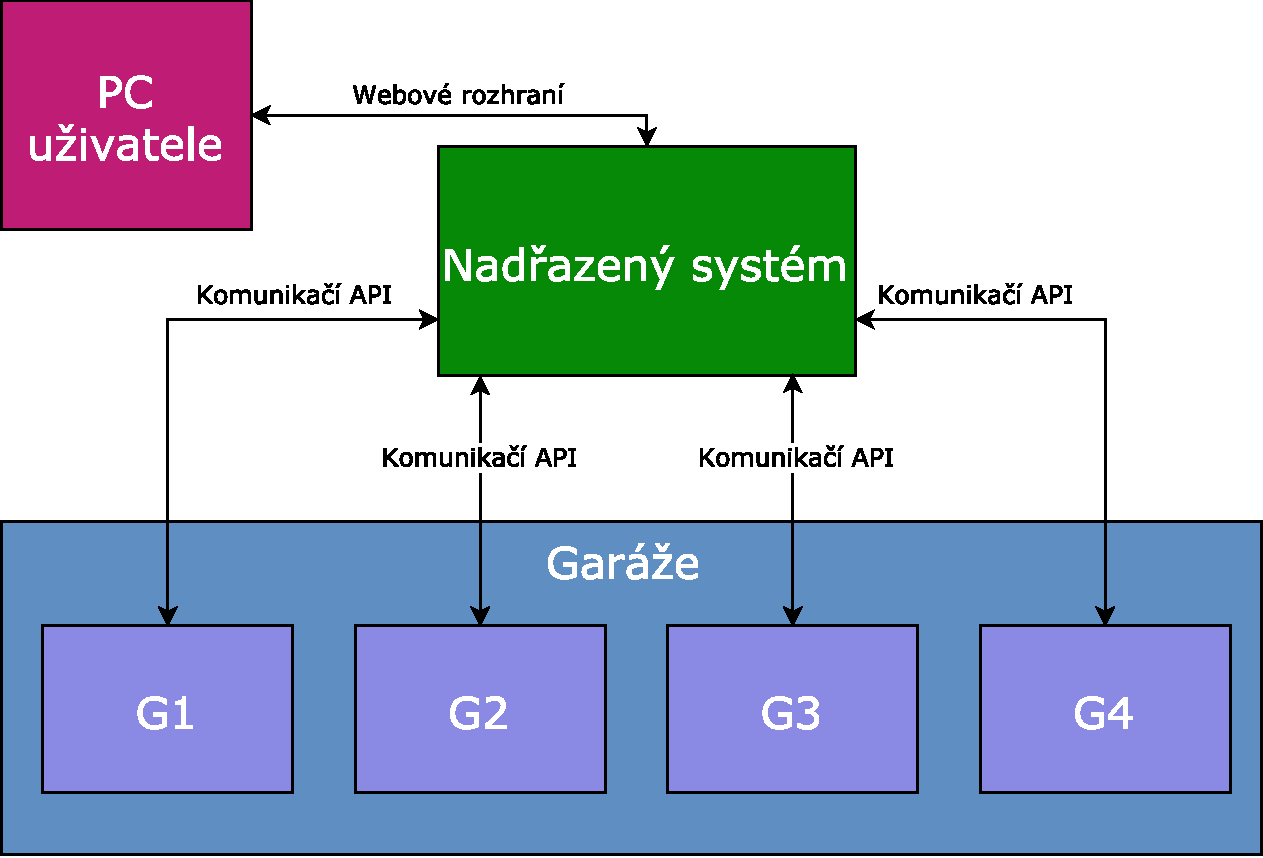
\includegraphics[width=\textwidth]{images/basic_struct.pdf}
    \caption[Základní struktura systému]{Základní struktura systému. Podřízené systémy využívají komunikační API k~zasílání událostí. Nadřazený systém tyto události zaznamenává a upravuje podle nich stav garáží. Uživatel nadřazený systém ovládá pomocí webového rozhraní. }
    \label{fig:basic_struct}
\end{figure}

\subsection{Podřízený systém}
\label{sec:an_subsystem}

Podřízený systém je zařízení umístěné v~každé garáži, které sleduje stav okolí pomocí těchto senzorových vstupů:

\begin{itemize}
    \item detekce kouře,
    \item detekce pohybu,
    \item stav dveří.
\end{itemize}

Základní požadavek na podřízený systém je schopnost komunikace přes Ethernet či WiFi pomocí protokolu zvoleného v~sekci \ref{sec:an_protocol}. Jinak může být hardware prakticky libovolný.

Návrh a implementace podřízeného systému není součástí této práce. Jeho vývojem se zabývá Miroslav Váňa ve své bakalářské práci na Katedře číslicového návrhu Fakulty informačních technologií ČVUT.

\subsection{Událost}

Událost slouží jako základní komunikační jednotka mezi nadřazeným a podřízeným systémem. V~případě překročení mezních hodnot senzorů se jednotlivé podřízené systémy okamžitě hlásí nadřazenému systému. Kromě toho také v~pravidelných intervalech odesílají kontrolní hlášení. 

Vyhodnocení události je provedeno nadřazeným systémem. Podřízený systém tedy hlásí každou událost (například otevření dveří), aniž by nějak zkoumal její závažnost.

\section{Výběr komunikačního protokolu}
\label{sec:an_protocol}

Nejdřív je nutné určit způsob komunikace, který bude systém používat. Díky tomu se budu při vybíraní platformy moci ujistit, že jsou dostupné vhodné knihovny a další software. 

Nadřazený systém bude se svými klienty (monitorovací zařízení v~jednotlivých garážích) komunikovat přes WiFi nebo Ethernet. Základem komunikace bude TCP/IP protokol \cite{tcp}, je však potřeba zvolit vhodný protokol z~aplikační vrstvy ISO OSI modelu \cite{tcp}, který na něm bude stavět.

\subsection{Vlastní protokol}

Jedna z~možností je implementovat vlastní protokol pomocí TCP/IP \textit{socketů}. Toto řešení se mi však nezdá příliš vhodné, neboť nepřináší žádné významné výhody, naopak se s~ním pojí řada komplikací.

Pro vlastní protokol by bylo nutné vytvořit robustní server, který zvládá obsluhu více klientů najednou. Dále by vzhledem k~citlivosti přenášených dat bylo nutné implementovat nějakou formu šifrování. Tyto velmi obsáhlé problémy přitom řeší většina dnešních protokolů.

Další nevýhodou je nutnost implementace klientské části protokolu při vytváření nových zařízení spravovaných nadřazeným systémem. To do jisté míry omezuje jeho rozšiřitelnost.

\subsection{Protokol HTTPS}
\label{sec:an_https}

Další možnost je využít ke komunikaci protokol HTTPS. V~tomto případě by klienti komunikovali se sytémem pomocí HTTP metod jako například \verb|get| nebo \verb|post|.

Jelikož součástí požadavků na systém je i webové uživatelské rozhraní, bude v~každém případě nutné použít webový server pro jeho provoz. Ten by pak bylo možné využít i k~poskytnutí API pro komunikaci systému s~podřízenými systémy.

Vhodný webový server (jako například Apache \cite{apache_faq}) zajistí vícevláknovou obsluhu všech klientů. Protokol se také postará o~šifrování přenášených dat, je však nutné získat certifikát k~ověření pravosti serveru (viz sekci \ref{sec:an_certs}).

Certifikát bude potřeba zajistit i v~případě, že komunikace s~klienty nebude postavena na tomto protokolu. Je totiž nutné také zabezpečit webové rozhraní, například kvůli ověření totožnosti uživatele při přihlašování. Nutnost pořízení certifikátu tedy nepředstavuje nevýhodu oproti jiným protokolům. 

API realizované pomocí tohoto protokolu je poměrně snadno rozšiřitelné. Pro nově implementovanou operaci stačí definovat URL a případně formát přenášených dat.

Výhodou je také snadná implementace na straně klienta, tedy podřízeného systému. Knihovny realizující klientskou část protokolu jsou dostupné na většině populárních platforem jako například Arduino (s~Ethernet \textit{shieldem}, oficiální knihovna EthernetClient \cite{ard_web}) nebo ESP8266 (knihovna esp8266wifi \cite{esp_web}).

\subsubsection{Certifikáty pro provoz HTTPS}
\label{sec:an_certs}

Pro provoz HTTPS serveru lze použít například certifikáty certifikační autority Let's Encrypt, které jsou poskytovány  zdarma \cite{lets_encrypt_faq}. Kromě toho dodává Let's Encrypt také automatizačního klienta Certbot \cite{certbot} pro snadné nasazení a aktualizaci jejich certifikátů. Bohužel certifikáty jsou vydávány pouze na doménu \cite{lets_encrypt_faq}, což komplikuje použití v~místní síti.

Jiná možnost je použití \textit{self-signed} certifikátu \cite{cert_wallen}. Tento certifikát není podepsaný žádnou certifikační autoritou, ale pouze vlastníkem certifikátu. Může tedy sloužit k~šifrování komunikace (poskytuje veřejný klíč), ale je zranitelný vůči \textit{man-in-the-middle} útoku \cite{cert_wallen}.

\textit{Self-signed} certifiát však lze použít k~šifrování komunikace na uzavřené lokální síti, za předpokladu, že je server s~certifikátem (přesněji s~jeho soukromým klíčem) dostatečně zabezpečen \cite{cert_wallen}. 

Nevýhodou tohoto řešení je nedůvěra webových klientů (certifikát není podepsán certifikační autoritou a nelze tedy ověřit jeho pravost), což by ovlivnilo přístup k~uživatelskému rozhraní a API systému. V~případě webového rozhraní by prohlížeč zobrazil varování o~neznámém certifikátu. To by však mohl uživatel ignorovat. 

Podřízené systémy by při zasílání požadavků museli přeskočit krok ověření totožnosti serveru. Jak toho dosáhnout například v~knihovně Requests (umožňující vytváření HTTP požadavků \cite{requests}) pro jazyk Python \cite{python_tutorial} je naznačeno v~ukázce \ref{lst:req_selfsigned}. 

Tento jazyk a knihovna byly zvoleny z~důvodů kompaktnosti ukázkového kódu, v~jiných jazycích lze tuto verifikaci obejít obdobným způsobem.

\begin{listing}[htbp]
\caption{\label{lst:req_selfsigned} Vytvoření HTTPS požadavku v~knihovně Requests, bez ověření totožnosti serveru.}
\begin{minted}[bgcolor=codebg]{python}
>>> import requests
>>> r = requests.get('https://test.local/hello', verify=False)
>>> r.status_code
200
\end{minted}
\end{listing}

\subsubsection{Autentizace klientů na HTTPS}

Přístup k~API nadřazeného systému by měl být povolen pouze ověřeným klientům. Díky tomu bude možné zabránit například zasílání nepravdivých informací z~neznámých zdrojů.

Jednoduchou autentizaci přes HTTPS lze realizovat například pomocí generování API klíčů. Pro každý podřízený systém bude vygenerován klíč, kterým se při zasílání požadavku systém prokáže. Seznam platných klíčů by byl udržován v~databázi nadřazeného systému. Klíče by uživatel mohl přidávat nebo odebírat (například v~případě odcizení podřízeného systému) pomocí webového rozhraní.

Tyto klíče by také bylo nutné nahrát a uchovávat na podřízených systémech. Detaily tohoto procesu by záležely na platformě těchto systémů. Například u~Arduina by šlo klíč nahrát z~uživatelova počítače pomocí sériové linky (s~USB převodníkem) a udržovat ho v~paměti EEPROM, která je uchována i po odpojení napájení \cite{ard_eeprom}.

Také by bylo možné implementovat v~nadřazeném systému \uv{registrační mód}, který by bylo možné dočasně povolit ve webovém rozhraní. V~tomto módu by systém po přijetí speciálního API požadavku vygeneroval nový klíč, který by si uložil do své databáze platných klíčů, a také ho v~odpovědi zaslal žádajícímu zařízení. Pokud by mód povolen nebyl, odpovědel by systém chybovým kódem, například \textit{403 -- Forbidden}. Zaslání požadavku z~podřízeného systému by mohlo být provedeno stisknutím tlačítka.

Tento přístup by byl pravděpodobně uživatelsky příjemnější, přináší však potencionální bezpečnostní rizika. Například pokud by uživatel zapomněl mód vypnout, systém by byl otevřený k~registraci nežádoucích zařízení. Takový problém by se však dal řešit například automatickou deaktivací módu po uplynutí časového limitu.

Útočník snažící se získat klíč k~API by také mohl periodicky zkoušet registrační požadavek a čekat na aktivaci módu. Obrana proti tomuto útoku by byla složitější, šlo by například filtrovat IP adresy s~příliš častými požadavky.

Obecně vycházím z~toho, že i v~případě registrace nežádoucího zařízení nemůže toto zařízení krátkodobě způsobit výraznější škody -- do databáze nadřazeného systému může pouze zasílat nová data, která jsou navíc vázana k~jeho identitě (API klíči). Nemůže tedy získávat data od jiných podřízených systému či měnit jejich záznamy. Neautorizované zařízení se také objeví v~seznamu registrovaných API klíčů, kde může být snadno odhaleno. 

\subsection{Protokol MQTT}
\label{sec:an_mqtt}

MQTT je komunikační protokol založený na modelu \textit{publisher/subscriber}, určený pro použití v~prostředí s~omezenými zdroji (malý výkon procesoru, omezená paměť atd.) \cite{mqtt_valerie}.

Komunikace mezi jednotlivými klienty v~systému je zprostředkována pomocí centrály nazývané \textit{broker}. Ta spravuje adresy -- \textit{topics}. Na nich mohou klienti publikovat či odebírat zprávy.

\begin{figure}[h!]
    \centering
    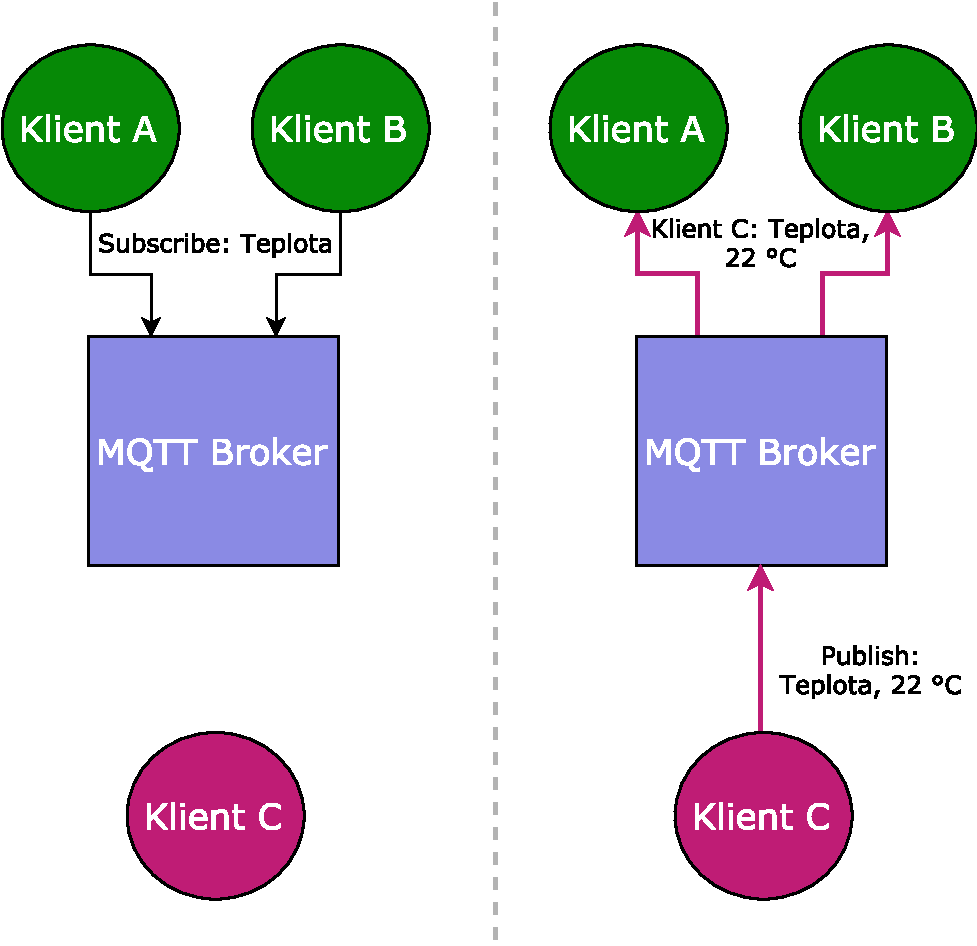
\includegraphics[width=\textwidth]{images/basic_mqtt.pdf}
    \caption[Příklad struktury protokolu MQTT]{Příklad struktury protokolu MQTT \cite{mqtt_eclipse}. Klienti A~a B jsou \textit{subscribery} \textit{topicu} \uv{Teplota}. Když klient C na tuto adresu publikuje novou zprávu, \textit{broker} se postará o~její doručení všem \textit{subscriberům}.}
    \label{fig:basic_mqtt}
\end{figure}

Na obrázku \ref{fig:basic_mqtt} tedy klienti \textcolor{green}{A} a \textcolor{green}{B} začnou odebírat \textit{topic} \uv{Teplota}. Když pak klient \textcolor{magenta}{C} pak publikuje zprávu na tuto adresu, \textcolor{blue2}{\textit{broker}} se postará o~doručení všem odebírajícím klientům.

Adresy je možné hierarchicky strukturovat následujícím způsobem \cite{mqtt_eclipse}: 

\begin{itemize}

\item Lze tvořit skupiny, například:
    \begin{itemize}
        \item \verb|/senzory/obyvak/teplota|.
        \item \verb|/senzory/kuchyne/vlhkost|.
    \end{itemize}
\item Zprávy je nutné publikovat na jednoznačnou adresu.
\item Při odebírání je možné použít modifikátory pro specifikování skupiny adres:
    \begin{itemize}
        \item Modifikátor \verb|+| -- odpovídá libovolnému jednomu stupni hierarchie. Například pro odebírání všech senzorů vlhkosti lze použít adresu \verb|/senzory/+/vlhkost|.
        \item Modifikátor \verb|#| -- odpovídá libovolnému počtu libovolných stupňů. Adresa \verb|/senzory/#| tedy slouží k~odebírání všech dat.
    \end{itemize}
\end{itemize}

V~případě této práce by tedy nadřazený systém i podřízené systémy byly klienty \textit{brokeru}. Podřízené systémy by publikovaly naměřená data, která by nadřazený systém odebíral. Tím by vznikla obdoba modelu \textit{client/server}, zmíněného v~sekci \ref{sec:an_struct}. 

Samotný \textit{broker} by pak mohl běžet souběžně s~nadřazeným systémem na zvolené platformě (například \textit{broker} Mosquitto je dostupný na řadě platforem, včetně Raspberry Pi \cite{mqtt_mosquitto_wiki}).

Protokol podporuje tři možnosti QoS \cite{mqtt_valerie}:

\begin{itemize}
    \item Nejvýše jedno doručení -- tento mód pouze odešle zprávu, není zahrnut žádný opakovací mechanismus pro případ nedoručení.
    \item Alespoň jedno doručení -- v~tomto módu je zaručeno doručení zprávy, ta však může být doručena vícekrát.
    \item Přesně jedno doručení -- zde je ošetřeno i duplicitní doručování zpráv.
\end{itemize}

Použití sofistikovanějších metod doručení má vliv na výkon, a proto se v~některých případech vyplatí zvolit nižší úroveň QoS (například při posílání idempotentních zpráv). Pro tuto práci bych však pravděpodobně zvolil záruku přesně jednoho doručení.

\subsubsection{Šifrování a autentizace na MQTT}

V~této části se budu zabývat prostředky pro šifrování komunikace, které jsou dostupné v~\textit{brokeru} Mosquitto.

První možnost je pro zabezpečení komunikace využít certifikáty, podobně jako u~HTTPS. Zde by se pravděpodobně také využil \textit{self-signed} certifikát (blíže popsaný v~sekci \ref{sec:an_certs}). Mosquitto navíc také vyžaduje kořenový certifikát certifikační autority \cite{mqtt_mosquitto_tsl}. Při použití \textit{self-signed} ceritifikátů by bylo nutné tuto autoritu vytvořit a používané certifikáty u~ní podepsat (pro bližší informace viz \cite{ca_nguyen}). Kořenový certifikát by také bylo nutné distribuovat klientům.

Kromě certifikátů lze pro šifrování použít i PSK. V~tom případě \textit{broker} a jeho klienti používají pro zašifrování komunikace společný klíč (známý jak klientovi, tak \textit{brokeru}). Různí klienti přitom mohou mít různé klíče. \cite{mqtt_mosquitto_conf}

Bohužel podpora PSK v~MQTT klientech není příliš rozšířená. PSK je možné použít v~knihovně libmosquitto, určené pro C/C++ (s~vazbami pro Python). U~této knihovny se mi však podařilo najít pouze manuálovou stránku (viz \cite{libmosquitto_man}), bez informací o~jejím dalším vývoji či udržování. Modul poskytující vazby do Pythonu byl nicméně předán projektu Paho \cite{mosquitto_python}.

Paho poskytuje implementace MQTT klientů pro mnoho platforem (včetně například Arduina \cite{paho_embedded}). Dokumentace klientů pro C++ a Python však možnost šifrování pomocí PSK vůbec nezmiňuje \cite{paho_cpp_doc, paho_pyt_doc}.

Tyto možnosti lze použít i k~autentizaci klientů \textit{brokeru}. Při použití certifikátů lze v~konfiguračním souboru Mosquitta zvolit \verb|require_certificate| \cite{mqtt_mosquitto_conf}. Poté bude od klienta vyžadován certifikát prokazující jeho totožnost. Při použití PSK lze k~autentizaci využít sdílený klíč (\textit{broker} odmítne klienty s~neplatnými klíči) \cite{mqtt_mosquitto_conf}. Kromě toho je možno použít také autentizaci pomocí uživatelského jména a hesla, která je součástí MQTT protokolu, případně totožnost klientů neověřovat vůbec (a pouze šifrovat komunikaci) \cite{mqtt_mosquitto_conf}.

\subsection{Závěr výběru protokolu}

V~sekcích \ref{sec:an_https} a \ref{sec:an_mqtt} jsem se blíže podíval na dva poměrně rozšířené protokoly aplikační vrstvy, které by bylo možné použít pro tvorbu nadřazeného systému.

Pokud by mezi požadavky na systém bylo zahrnuto zasílání nevyžádaných zpráv podřízeným systému (jak je zmíněno v~sekci \ref{sec:an_struct}), zvolil bych pravděpodobně protokol MQTT. V~něm je tato funkcionalita velmi snadno implementovatelná -- stačí, aby podřízené systémy odebíraly \textit{topic}, na kterém by nadřazený systém publikoval zprávy.

Jelikož se však v~této práci zabývám systémem, který zprávy pouze přijímá a zaznamenává, rozhodl jsem se pro HTTPS. Nasazení tohoto protokolu je o~něco snazší (není potřeba na zařízení instalovat \textit{broker} a zařizovat certifikační autoritu -- stačí \textit{self-signed} certifikát) a s~jeho použitím mám více zkušeností. Také se částečně uvolní požadavky na volbu platformy (webový server bude potřeba v~každém případě, při volbě HTTPS jako komunikačního protokolu mezi systémy tedy nebude nutný žádný další software). 

Každopádně bude mým cílem navrhnout výslednou aplikaci tak, aby rozhraní pro podřízené systémy realizované pomocí HTTPS bylo možné snadno nahradit MQTT rozhraním.

K~zabezpečení komunikace (včetně webového rozhraní) použiju \textit{self-signed} certifikát. Hlavní důvod je požadavek na použití v~místní síti, bez zaručeného přístupu k~internetu. Toto rozhodnutí nemá vliv na návrh a implementaci systému, pouze na jeho nasazení -- konkrétně konfiguraci webového serveru.

Pokud by provozovatel plánoval mít systém přístupný z~internetu (přes registrovanou doménu), musí v~každém případě k~zabezpečení použít certifikát podepsaný důvěryhodnou certifikační autoritou. Pak stačí pouze v~konfiguračním souboru webového serveru nahradit \textit{self-signed} certifikát podepsaným certifikátem. Není tedy nutné provádět změny v~kódu aplikace.

\section{Ukládání dat}
\label{sec:an_data}

Zaznamenané události bude potřeba presistentně uchovávat. Zde by šly využít jednoduché textové logy, vhodnější však bude zvolit nějaký databázový systém -- například kvůli širším možnostem zpracování naměřených údajů.

Z~dostupných možností mě zaujal SQLite, což není klasický databázový stroj s~modelem \textit{client/server}, ale místo toho tvoří součást programu, který databázi používá. Přístup k~datům je realizován pomocí přímého čtení/zápisu do databázového souboru na disku.  Díky tomu má malé nároky na diskový prostor a operační paměť. \cite{sqlite_about}

Jelikož bude nadřazený systém pravděpodobně provozován na hardwaru s~omezenými zdroji, představují tyto vlastnosti nezanedbatelnou výhodu. Použití SQLite také zjednouší nasazení aplikace, neboť nebude nutné vytvářet a konfigurovat databázový server.

\subsection{Velikost databáze}

Vzhledem k~požadavku na spolehlivost systému je vhodné odhadnout předpokládaný růst velikosti databázového souboru. Přiliš velká databáze by mohla vyčerpat pamět zařízení, a způsobit tak jeho pád. Také by mohla negativně ovlivnit dobu odezvy nadřazeného systému.

Pokud by se ukázalo, že při dlouhodobém provozu začíná být databáze neúnosně velká, bylo by nutné omezit množství uchovávaných dat, například pomocí front zaznamenaných událostí.

Při odhadu jsem vycházel z~předpokladu, že největší objem dat v~databázi budou představovat zaznamenaná kontrolní hlášení podřízených systému. Pokud se budou podřízené systémy hlásit každou hodinu, představuje to 24 záznamů denně na každou garáž, což by mělo být řádově více než u~jiných událostí. Například u~pravděpodobně druhé nejčastější události, tedy otevření/zavření dveří, předpokládám nejvýše jednotky denně.

Událost kontrolního hlášení by měla obsahovat tyto údaje:

\begin{itemize}
    \item Identifikátor události v~databázi.
    \item Identifikátor garáže, ke které událost patří.
    \item Datum a čas zaznamenání události.
    \item Typ události (kontrolní hlášení).
\end{itemize}

Identifikátory a typ události pravděpodobně budou 32bitová celá čísla. Datum je možné v~SQLite ukládat buď jako textový retězec ve formátu \texttt{YYYY-MM-DD HH:MM:SS.SSS}, 64bitové reálné číslo, či 32bitové cele číslo -- \textit{Unix Time} \cite{sqlite_datetypes}. Z~toho vyplývá, že jedno kontrolní hlášení bude mít velikost alespoň $4 \cdot 32 = 128$ bitů.

Pokud nadřazený systém monitoruje 30 garáží, přičemž každá odesílá kontrolní hlášení každou hodinu, jsou každý den vytvořeny záznamy o~velikosti $30 \cdot 24 \cdot 96 = 98304$ bitů, tedy asi 98 Kb. Dá se tedy předpokládat, že velikost databázového souboru neporoste nijak dramaticky.

Tento výpočet představuje pouze odhad předpokládané velikosti. Skutečná velikost bude záležet na zvolené implementaci, neměla by se však výrazně lišit od tohoto odhadu.

%v implementaci este popsat zmeny voproti tomuhle vodhadu, mozna taky doplnit aktualizovanej vypocet

\section{Zasílání upozornění}
\label{sec:an_notify}

Nadřazený systém má být schopen zasílat uživatelům notifikace o~stavu jednotlivých garáží. Notifikace mohou informovat o~důležité události (například detekce kouře) nebo o~výpadku podřízeného systému (v~případě promeškání plánovaného kontrolního hlášení).

Tyto notifikace by měl obdržet jednak správce garáží (provozovatel nadřazeného systému), jednak jednotliví nájemci, kterým budou zasílány notifikace týkající se jejich garáží.

V~následujících sekcích jsem otestoval několik přístupů k~odesílání těchto notifikací, a to jak pomocí e-mailu tak SMS.

\subsection{E-mailové notifikace}

První možnost je zasílat notifikace pomocí e-mailu. K~tomu je zapotřebí vytvořit účet, který by mohl nadřazený systém použít k~odesílání.

Zde se nabízí možnost provozovat e-mailový server s~účtem přímo na zařízení, na kterém poběží nadřazený systém. Provoz takového serveru je však velmi náročný, a to nejen kvůli složité počáteční konfiguraci, ale také z~hlediska dlouhodobé údržby \cite{email_dont}. Tento přístup by tak kladl neúměrné nároky na uživatele systému.

Alternativa je použít nějakého poskytovatele e-mailových služeb, jako například Gmail od společnosti Google. Zde by si uživatel vytvořil účet určený k~odesílání notifikací, a poté autorizoval nadřazený systém k~odesílání zpráv z~tohoto účtu. 

Tímto je částečně porušen požadavek na nezávislost (viz sekci \ref{sec:an}). Při zasílání notifikací je však nutný přístup k~internetu i v~případě použití vlastního e-mailového serveru a nezávislost na externí službě nevyváží komplikace spojené s~jeho provozem.

Gmail umožňuje přístup k~účtu pomocí SMTP, je však nutné v~nastavení účtu Google povolit přístup méně zabezpečeným aplikacím, protože přihlášení je prováděno pomocí uživatelského jména a hesla \cite{google_smtp}. Jelikož by příhlašovací údaje musely být uloženy v~nadřazeném systému v~čitelné podobě, není tento způsob vhodný.

Bezpečnější možnost je použít k~přístupu protokol OAuth2 \cite{rfc6749}. S~jeho pomocí je možné udělovat aplikacím (v~tomto případě nadřazenému systému) přístup k~částem účtu Google, tedy i Gmailu. Autentizace probíhá na základě náhodně generovaných klíčů, není tedy nutné uchovávat v~nadřazeném systému heslo, které mohl uživatel systému použít i v~jiných službách, v~čitelné podobě \cite{google_oauth}.

% este by se dalo napsat ze timhle taky de vomezit k jaky casti toho google uctu bude mit ten token pristup

\subsection{SMS notifikace}

Alternativa k~e-mailu je posílání upozornění pomocí SMS. To může být pro uživatele vhodnější, protože lze upozornění přijímat na prakticky jakémkoliv telefonu, bez nutnosti e-mailového klienta či připojení k~internetu.

Posílání SMS z~nadřazeného systému lze provést dvěma způsoby. První možnost je připojit k~počítači, na kterém nadřazený systém poběží, GSM modul se SIM kartou. Také je možné k~posílání SMS využít internetovou službu, jako je například Twilio.

\subsubsection{GSM modul}

Poměrně snadný způsob jak odeslat SMS pomocí počítače je využít GSM modul, který lze připojit do USB (například modul E3131 od společnosti Huawei, zobrazený na obrázku \ref{fig:gsm_module}). Počítač může s~modulem komunikovat pomocí sériové linky a příkazů, které definuje GSM standard \cite{gsm_standard}. Díky tomu nejsou nutné specializované ovladače a modul lze použít na mnoha různých zařízení.

Modul je možné ovládat přímo pomocí sériové linky, vhodnější je však použít program či knihovnu, která zařídí zasílání příslušných příkazů. To je například projekt Gammu, který umožňuje komplexní ovládání modulu buď pomocí příkazové řádky nebo knihovny v~jazyce C \cite{gammu}.

\begin{figure}[h!]
    \centering
    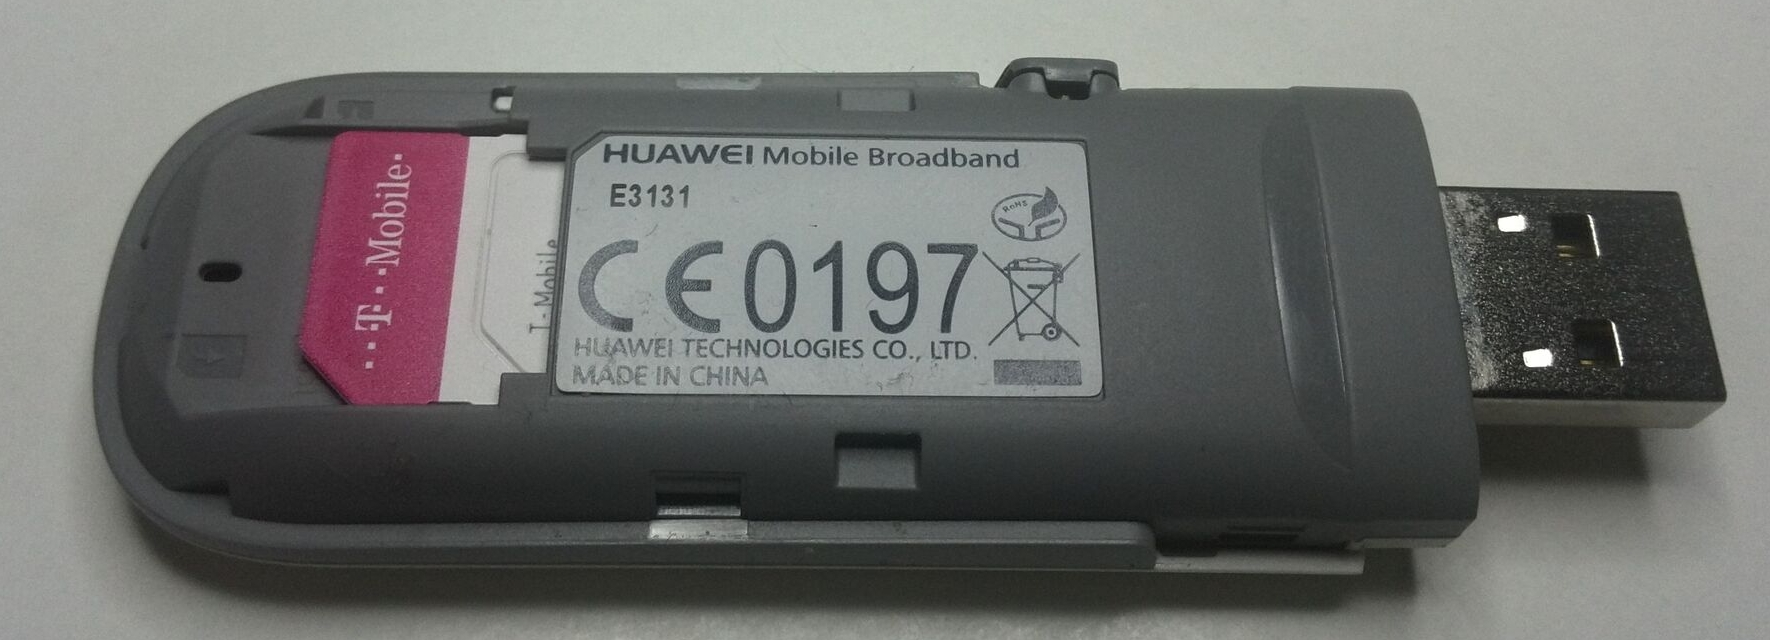
\includegraphics[width=\textwidth]{images/gsm_module.jpg}
    \caption[GSM modul Huawei E3131]{GSM modul Huawei E3131 s~odkrytým slotem pro SIM kartu.}
    \label{fig:gsm_module}
\end{figure}

Výhoda tohoto řešení je nezávislost na internetu. Odesílání upozornění by tedy fungovalo i pokud by zařízení mělo přístup pouze k~místní síti. Řešení je také poměrně snadno implementované (po připojení modulu a instalaci knihovny stačí k~odeslání SMS jediný příkaz) a díky jednoduchému komunikačnímu rozhraní modulu výrazně neomezuje požadavky na hardware či ovladače.

Za hlavní nevýhodu považuji cenu řešení. Jednak je potřeba pořídit GSM modul, jednak je nutné platit odeslané SMS (zde by záleželo na zvoleném tarifu). Méně významné nevýhody představují nutnost udržovat v~modulu aktivní SIM kartu a případně dostatečný kredit.

%v tim gammu pouzit https://wammu.eu/docs/manual/smsd/usage.html#creating-messages-to-send daemona to vyresi problemy s dlouho trvajicim vodeslanim a taky asi se sudo pristupem, tohle popsat v implementaci

%cool moznost -- vlastni gsm modul, vyhody -- hlavne nezavislost (de i bez netu), kompatibilni s hafem hw (staci seriova linka, komunikace pomoci at commandu), knihovny/programy (gammu) pro snadny vovladani. nejde posilat smsky bez toho gsm modulu, tj nestaci vopsat api klice jako u twilio. nevyhody -- spatna kontrola (kredit -- jako cist kredit asi de nak pres ty ussd zpravy ale celej ten interface by se musel naprogramovat a v tim twilliu je proste uz hotovej, varovani vo zruseni simky atd), nutnost mit ten modul (nefungovalo by pri nasazeni v cloudu), muze bejt relativne drahej (jak modul tak samotny sms), nutnost sehnat simku, pri zruseni simky problem zjistit ze se to stalo, gammu nema knihovnu pro python3

\subsubsection{Twilio}

K~odesílání SMS lze také využít službu Twilio, která umožňuje registraci telefonního čísla a posílání SMS pomocí webového API \cite{twilio_sms}. K~tomu lze použít připravenou knihovnu pro Python \cite{twilio_python}. Přístup k~API je ověřen pomocí klíčů, které uživatel obdrží po registraci \cite{twilio_keys}.

Toto řešení je levnější než řešení využívající GSM modul, neboť není nutné kupovat žádný další hardware. Samotné odesílání SMS je také poměrně levné -- jedna zpráva odeslaná v~rámci České republiky přijde na 0.049 USD \cite{twilio_pricing}. Kromě toho Twilio poskytuje další služby, které by bylo možné použít k~budoucímu rozšíření nadřazeného systému \cite{twilio_products}.

Nevýhoda může být (stejně jako u~řešení založeného na e-mailech) nutnost připojení k~internetu a registrace účtu. Kromě toho je nutné na účtu udržovat kredit k~odesílání SMS, což vyžaduje zadání platební karty.

%dalsi moznost twilio -- sluzba na posilani sms. vyhody -- relativne jednoduchy pouziti, snadna kontrola nad utratou, naky fancy pokrocily moznosti (custom cisla atd), levny (smsky, neni potreba gsm modul), comfy knihovna pro python3, snadna implementace, je mozny to pouzit i v tim cloudu. nevyhody -- potrebuje internet, nutna registrace (+ vyplneni kreditni karty, ale srovnat se shanenim sim karty), (trosicku slozitejsi na pouziti pro uzivatele -- musi vyplnit tri veci v tim web rozhrani). este teda je blby ze kdo ma pristup k tomu rpi muze posilat smsky vodkudkoliv kdyz si vopise ten auth token

% naky zajimavy info https://support.twilio.com/hc/en-us/articles/223181828-Does-Twilio-check-to-see-if-phone-numbers-can-receive-SMS-

%https://support.twilio.com/hc/en-us/articles/223183228-How-Does-Twilio-s-Pricing-Work-

% gammu kredit> sudo gammu --getussd AA182C3602 #to AA.. je zakodovany *101#

\subsection{Závěř výběru způsobu zasílání upozornění}

Po otestování výše zmíněných metod zasílání upozornění jsem se rozhodl použít GSM modul. Hlavní důvod pro toto rozhodnutí byla vyšší nezávislost nadřazeného systému (není potřeba internetové připojení) a poměrně snadná implementace. 

Zasílání upozornění pomocí SMS se mi zdá vhodnější než pomocí e-mailu. E-mail může být pro uživatele hůře dostupný -- k~jeho kontrole potřebuje vhodný telefon či počítač s~připojením k~internetu. Příchozí SMS je také snazší vzít na vědomí.

\section{Programovací jazyk pro tvorbu systému}
\label{sec:an_lang}

Pro tvorbu systému jsem se rozhodl použít programovací jazyk Python \cite{python_tutorial}. S~tímto jazykem mám nejvíce zkušeností co se týče implementace webových aplikací. Je také dostatečně rozšířený, takže výsledný systém bude možné nasadit na poměrně širokém spektru platforem bez nutnosti složitějšího portování.

K~vytvoření webového rozhraní i API pro podřízené systémy jsem zvolil framework Flask \cite{flask_about}. Hlavní důvod jsou opět předchozí zkušenosti s~tímto frameworkem. Flask také dává více volnosti při návrhu aplikace než například také velmi rozšířený framework Django \cite{django_about}.

\section{Výběr platformy}
\label{sec:an_plat}

Pro realizaci systému je nutné zvolit vhodnou platformu. Jelikož je cílem práce vytvořit fyzické zařízení, rozhodl jsem se jako základ použít některý z~jednodeskových počítačů, které jsou v~dnešní době na trhu. Tyto počítače bývají cenově velmi dostupné a zároveň poskytují dostatečný výkon a podporu pro provoz systému.

Při výběru počítače byla nejdůležitejším kritériem podpora softwaru potřebného k~implementaci monitorovacího systému. Na základě předchozí analýzy je tedy vyžadován následující software:

\begin{itemize}
    \item Webový server Apache2.
    \item Databázový systém SQLite3.
    \item Programovací jazyk Python3.
    \begin{itemize}
        \item Webový framework Flask.
    \end{itemize}
\end{itemize}

Pro provoz tohoto softwaru bude potřeba plnohodnotný operační systém, což vylučuje platformy využívající jednoduché mikrokontroléry, jako například Arduino Uno. Kromě toho je nutné připojení k~síti pomocí Ethernetu nebo WiFi. 

V~dalších sekcích jsem se blíže podíval na jednodeskové počítače Raspberry Pi (sekce \ref{sec:an_rpi}) a Zybo Zynq-7000 (sekce \ref{sec:an_zyb}) a zvážil jejich výhody a nevýhody pro implementaci systému.

\subsection{Raspberry Pi}
\label{sec:an_rpi}

\begin{figure}[h!]
    \centering
    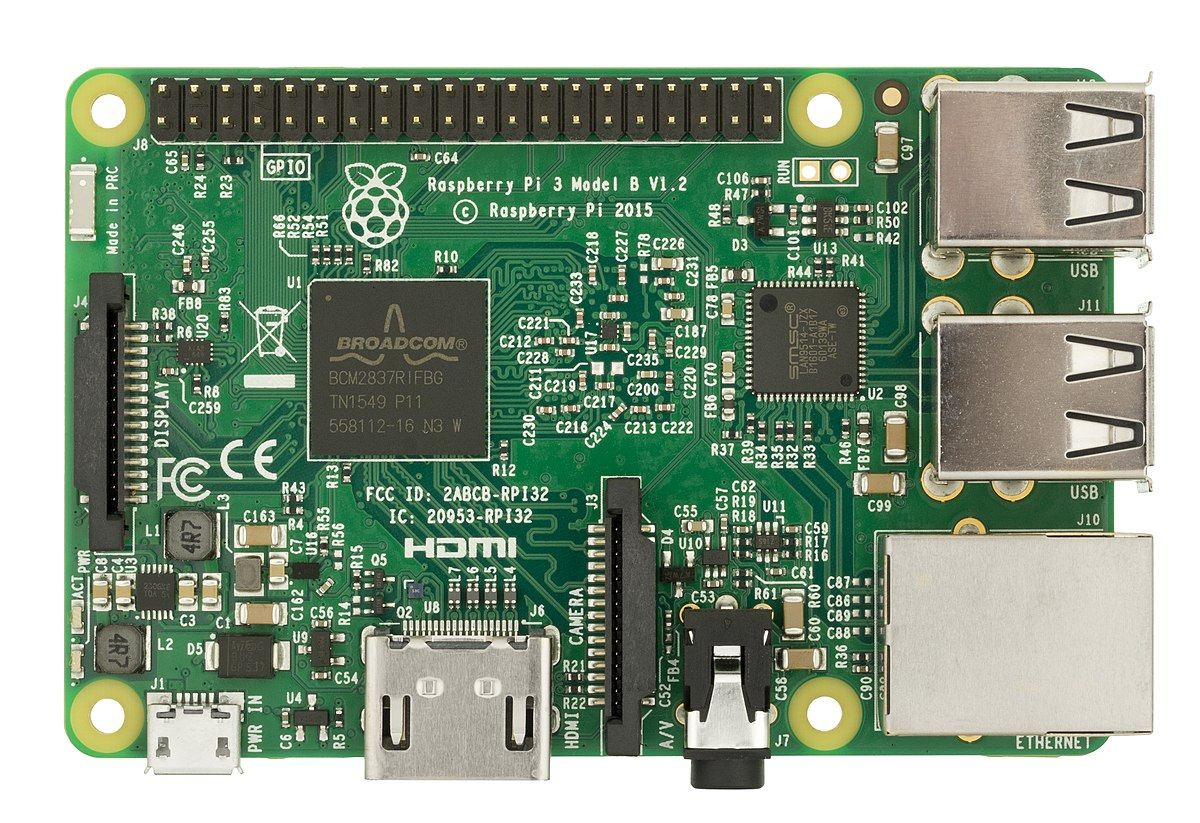
\includegraphics[width=0.7\textwidth]{images/rpi.jpg}
    \caption[Raspberry Pi 3]{Raspberry Pi 3 (obrázek převzat z~\url{https://en.wikipedia.org/wiki/Raspberry_Pi}).}
    \label{fig:rpi}
\end{figure}

Raspberry Pi je velmi rozšířený jednodeskový počítač. Jeho poslední verze, Raspberry Pi 3, je postavena na SoC Broadcom BCM2837 s~čtyřjádrovým procesorem ARM Cortex A53, který je až o~50 \% rychlejší než procesor předchozí verze \cite{rpi_benchoff}.

Dále nová verze přináší vlastní WiFi modul \cite{rpi_benchoff}, není tedy nutné se spoléhat na externí moduly. Kromě toho je možné počítač připojit k~síti pomocí Ethernetového portu. Ten je omezený na 100 Mb/s \cite{rpi_benchoff}, to by však vzhledem k~objemu dat přenášených mezi nadřazeným a podřízenými systémy nemělo představovat problém.

Deska také obsahuje čtyři USB a jeden HDMI port \cite{rpi_benchoff}. Ty nejsou pro implementovaný systém zásadní, nicméně při počáteční konfiguraci zařízení (například nastavení WiFi hesla) může být připojení monitoru a klávesnice pro některé uživatele pohodlnější než použití SSH či sériové linky. Připojený monitor se také hodí při řešení problémů se startem operačního systému.

Raspberry Pi 3 bohužel nemá vlastní bateriově zálohovaný RTC obvod a k~udržování času využívá protokol NTP \cite{rpi_rtc_ada}. K~tomu je však zapotřebí internetové připojení. Jelikož by zařízení mělo být možné používat i v~síti bez přístupu k~internetu, je nutné připojit externí RTC obvod, napřílad pomocí I2C sběrnice \cite{rpi_rtc_ada}. Poté je možné systémové hodiny synchronizovat bez internetového připojení pomocí tohoto obvodu.

S~počítačem je možné použít množství operačních systémů, z~nichž nejrozšířenější je pravděpodobně Raspbian, linuxový systém postavený na Debianu \cite{raspbian_faq}. Pro ten jsou dostupné všchny potřebné softwarové balíčky popsané v~sekci \ref{sec:an_plat}. Jelikož počítač nemá žádné vlastní úložiště, je nutné operační systém provozovat na vložené SD kartě \cite{rpi_benchoff}.

Jednou z~výhod tohoto počítače je obrovské množství podporovaných hardwarových periferií a knihoven pro ně. V~této práci bych využil pouze zmíněný RTC obvod, případné další rozšiřování systému (například o~vestavěný LCD displej) bude na Raspberry Pi pravděpodobně snadnější než na jiných platformách.

Kromě široké podpory je hlavní výhodou Raspberry Pi jeho cena. Poslední verze se pohybuje kolem 1200 Kč. K~celkovým nákladům na systém je ještě třeba připočítat cenu RTC obvodu a SD karty. Zde počítám s~použitím již připraveného modulu s~obvodem PCF8523 (pro bližší informace o~modulu viz \cite{rpi_rtc_ada}), jehož cena je příbližně 200 Kč. Jako úložiště by měla plně dostačovat 16GB SD karta, která se dá pořídit za 200 Kč. Celkové náklady na hardware systému se tedy měly pohybovat kolem 1600 Kč\footnote{Ceny převzaté z~obchodů Alza (\url{https://alza.cz}) a SnailShop (\url{www.snailshop.cz}), v~únoru 2018.}.

\subsection{Zybo Zynq-7000}
\label{sec:an_zyb}

\begin{figure}[h!]
    \centering
    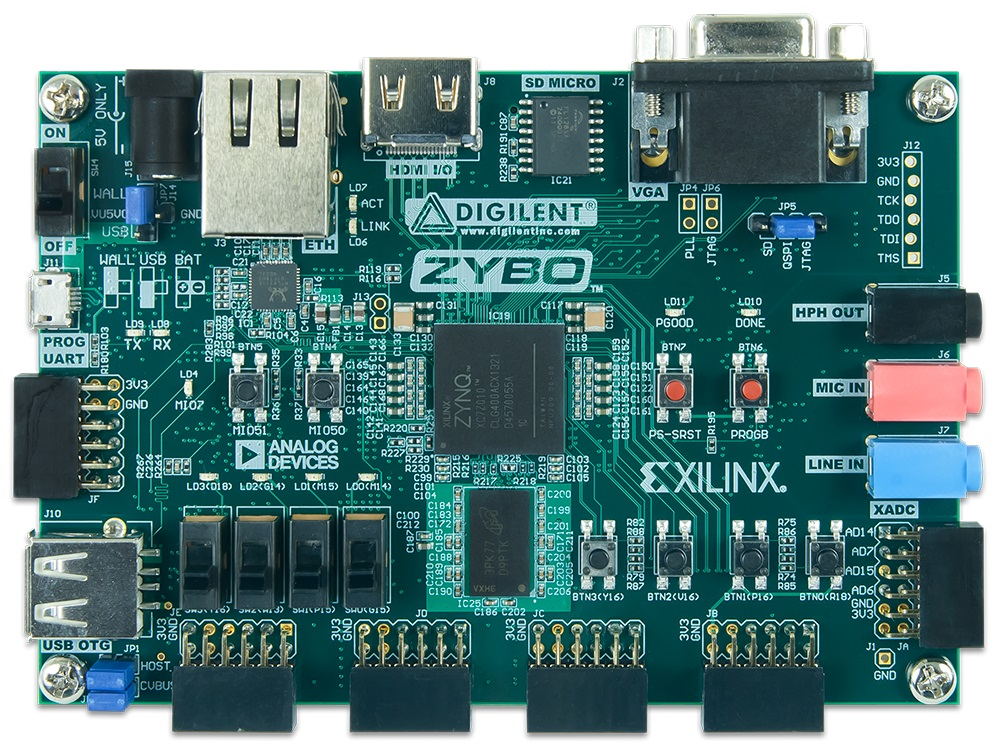
\includegraphics[width=0.7\textwidth]{images/zybo.jpg}
    \caption[Přípravek Zybo Zynq-7000]{Připravek Zybo Zynq-7000 (obrázek převzat z~\url{https://www.xilinx.com/products/boards-and-kits/1-4azfte.html}).}
    \label{fig:zybo}
\end{figure}

Tento přípravek od společnosti Digilent je postavený na SoC Xilinx Zynq Z-7010. Hlavní předností tohoto čipu je kombinace dvoujádrového procesoru ARM Cortex A9 s~FPGA odpovídající sérii Artix-7 \cite{zybo_man}. 

Díky tomu je možná těsná integrace mezi aplikací běžící na procesoru a výkonnými, úzce specializovanými moduly, které jsou syntetizované na FPGA. Tento přístup, kdy je hardware a software systému vyvíjen souběžně se označuje jako \textit{hardware/software codesign} \cite{hw_code}.

%dostupne operacni systemy -- petalinux, xilinux
Pro SoC ze série Zynq vznikla linuxová distribuce Xilinux, vycházející z~Ubuntu. Kromě plnohodnotného operačního systému (včetně například grafického rozhraní) poskytuje Xilinux také ovladače pro komunikaci s~FPGA pomocí AXI sběrnice \cite{xilibus}. K~tomu využívá \textcolor{magenta}{IP jádro Xilibus}, které funguje jako adaptér mezi \textcolor{green}{procesorem} a FPGA modulem (viz obrázek \ref{fig:xilibus}). Ten pak ke komunikaci může využívat standardni \textcolor{blue2}{FIFO} fronty a nemusí se zabývat AXI sběrnicí \cite{xilibus}.

\begin{figure}[h!]
    \centering
    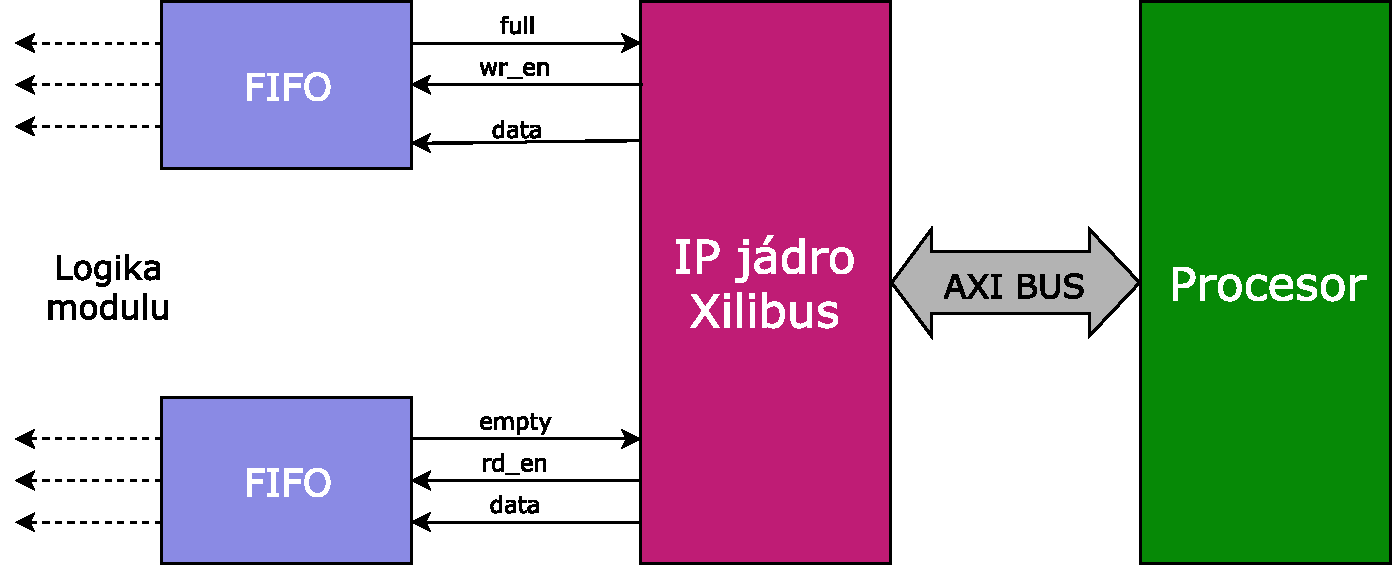
\includegraphics[width=\textwidth]{images/xilibus.pdf}
    \caption[Blokové schéma využití IP jádra Xilibus]{Blokové schéma využití IP jádra Xilibus \cite{xilibus}. Procesor přípravku komunikuje pomocí AXI sběrnice s~jádrem Xilibus. To požadovaná data zapíše či přečte z~FIFO fronty příslušného modulu.}
    \label{fig:xilibus}
\end{figure}

Jelikož Xilinux staví na Ubuntu (konkrétně na verzi 12.04 LTS \cite{xilibus}), neměl by být problém nainstalovat software potřebný pro provoz nadřazeného systému (viz sekci \ref{sec:an_plat}). 

Přípravek je možné připojit k~síti pomocí ethernetového portu, který podporuje rychlost až 1 Gb/s \cite{zybo_man}. WiFi připojení by bylo možné realizovat pomocí USB modulu. Dále přípravek obsahuje HDMI a VGA port, audio konektory, čtyři tlačítka, čtyři přepínače a slot pro SD kartu \cite{zybo_man}.

Na přípravku je také k~dispozici 128 MB flash paměti \cite{zybo_man}, k~provozu tedy teoreticky není potřeba SD karta. Tato paměť by však pravděpodobně nestačila k~instalaci vhodného operačního systému a potřebného softwaru. I~zde by tedy bylo nutné použít SD kartu.

Stejně jako Raspberry Pi tato deska postrádá RTC obvod. Firma Digilent však dodává externí obvod, který lze připojit pomocí Pmod rozhraní \cite{pmod_rtc_man}. 

Nevýhodu této desky (především v~porovnání Raspberry Pi) je její cena. Ta se pohybuje okolo 4000 Kč\footnote{Cena podle produktové stránky \url{https://www.xilinx.com/products/boards-and-kits/1-4azfte.html}, v~únoru 2018.}. K~tomu je nutné přičíst náklady na SD kartu a RTC obvod, případně i WiFi modul. Cena celého zařízení by se tedy pohybovala v~rozmezí 4500 až 5000 Kč.

%bacha tady este na "As of 9/21/2017- the Zybo will be replaced by the Zybo Z7-10. We have created this guide to help you migrate your designs to the Zybo Z7. " ale nevim jestli to ma cenu resit ty desky se lisej minimalne (SoC je stejnej)
%^^linx: https://store.digilentinc.com/zybo-z7-zynq-7000-arm-fpga-soc-development-board/

\subsection{Závěr výberu platformy}

\begin{table}[h!]
\centering
\begin{tabular}{|c | c | c |} 
 \hline
 & \textbf{Raspberry Pi 3} & \textbf{Zybo Zynq-7000} \\
 \hline 
 SoC & Broadcom BCM2837 & Xilinx Zynq Z-7010 \\ 
 Procesor & ARM Cortex A53 & ARM Cortex A9 \\
 & 4 jádra, 1.2 GHz & 2 jádra, 650 MHz \\
 RAM & 1024 MB LPDDR2 & 512 MB DDR3 \\
 FPGA & -- & ekvivalent řady Artix-7 \\
 Úložiště & SD karta & 128 MB Flash, SD karta \\
 Síť & 100 Mb/s Ethernet, WiFi & až 1 Gb/s Ethernet \\
 Cena & 1200 Kč & 4000 Kč \\
 \hline
\end{tabular}
\caption[Srovnání platforem Raspberry Pi 3 a Zybo Zynq-7000]{Srovnání platforem Raspberry Pi 3 a Zybo Zynq-7000 \cite{rpi_benchoff, zybo_man}.}
\label{tab:plat_compare}
\end{table}

Jak vyplývá z~tabulky \ref{tab:plat_compare}, Raspberry Pi 3 poskytuje znatelně výkonnější procesor a více paměti za méně než třetinu ceny desky Zybo. Hlavní přidaná hodnota Zybo tedy spočívá v~integraci s~FPGA, ta má však v~případě této práce pouze velmi omezené využití. 

FPGA by bylo možné využít například k~šifrování úložiště, vzhledem k~předpokládáným objemům dat by však zrychlení oproti softwarovému šifrování neospravedlnilo vysokou cenu přípravku. Na druhou stranu vyšší výkon procesoru u~Raspberry Pi může mít pro nadřazený systém význam, například z~hlediska odezvy uživatelského rozhraní.

Jako platformu pro implementaci nadřazeného systému jsem tedy zvolil Raspberry Pi 3, především kvůli příznivé ceně, výrazně lepšímu poměru cena/výkon (pro tuto práci), a také kvůli podpoře a rozšiřitelnosti.

\subsection{Provoz aplikace na \textit{cloudové} platformě}
\label{sec:an_cloud}

V~této části bych chtěl popsat alternativu k~provozu systému na dedikovaném zařízení, a to možnost využít virtuální server na některé \textit{cloudové} platformě. Primární cíl práce je sice vytvořit nadřazený systém jako jednoúčelové zařízení (postavené na Raspberry Pi), nicméně provoz výsledné aplikace v~\textit{cloudu} může být v~určitých situacích vhodnější řešení.

Jedním z~možných uplatnění této varianty je monitorování více garážových komplexů. Místo lokálního nadřazeného systému by mohly všechny \textcolor{blue2}{podřízené systémy} z~každého komplexu komunikovat s~jedním \textcolor{magenta}{globálním systémem}, provozovaným na virtuálním serveru a dostupným z~internetu, jak je naznačeno na obrázku \ref{fig:aws}. Při tomto provozu je však nutnost mít registrovanou doménu a zabezpečit spojení podepsaným certifikátem.

Virtuální servery nabízí například firma DigitalOcean. Cena serveru závisí na počtu výpočetních jader, dostupné RAM a velikosti úložiště. Nejlevnější konfigurace stojí 5 USD měsíčně a nabízí jednojádrový procesor, 1 GB RAM a 25 GB SSD \cite{digi_pricing}. Předpokládám, že tento výkon by stačil pro základní provoz systému, v~případě vyššího počtu podřízených systémů je však možnost zvyšovat dostupnou paměť a přidávat procesorová jádra. 

S~těmito virtuálními servery lze použít řadu běžných linuxových operačních systémů jako Ubuntu, Debian či Fedora \cite{digi_droplets}, dostupnost softwaru potřebného pro spuštění aplikace tedy není problém.

Hlavní nevýhodou tohoto přístupu je poněkud složitější nasazení a spuštění systému. Registrace domény, získání certifikátu a základní konfigurace webového serveru se dá sice částečně automatizovat (viz zmiňovaný Certbot \cite{certbot}), pro většinu uživatelů bude však pravděpodobně snazší použít již připravené Raspberry Pi.

Také je složitější distribuovat adresu serveru s~nadřazeným systémem podřízeným systémům. V~místní síti může podřízený systém sám nalézt nadřazený systém testováním odpovědi zařízení v~síti na registrační požadavek. Pokud by však byl nadřazený systém dostupný pouze na internetové doméně, bylo by nutné ji ručně zadat každému podřízenému systému.

Další problém může představovat hlavní výhoda tohoto řešení, a to přístupnost serveru z~internetu. Ta významně zvyšuje \textit{attack surface} celého nadřazeného systému, zvlášt oproti alternativě využívající k~propojení systémů pouze Ethernet, u~kterého má (na rozdíl od WiFi) provozovatel fyzický přehled o~připojených zařízeních.

Při nasazení na virtuálním serveru také nelze použít GSM modul. Pro posílání upozornění by tak bylo nutné zvolit jiný způsob, například službu Twilio.

\begin{figure}[h!]
    \centering
    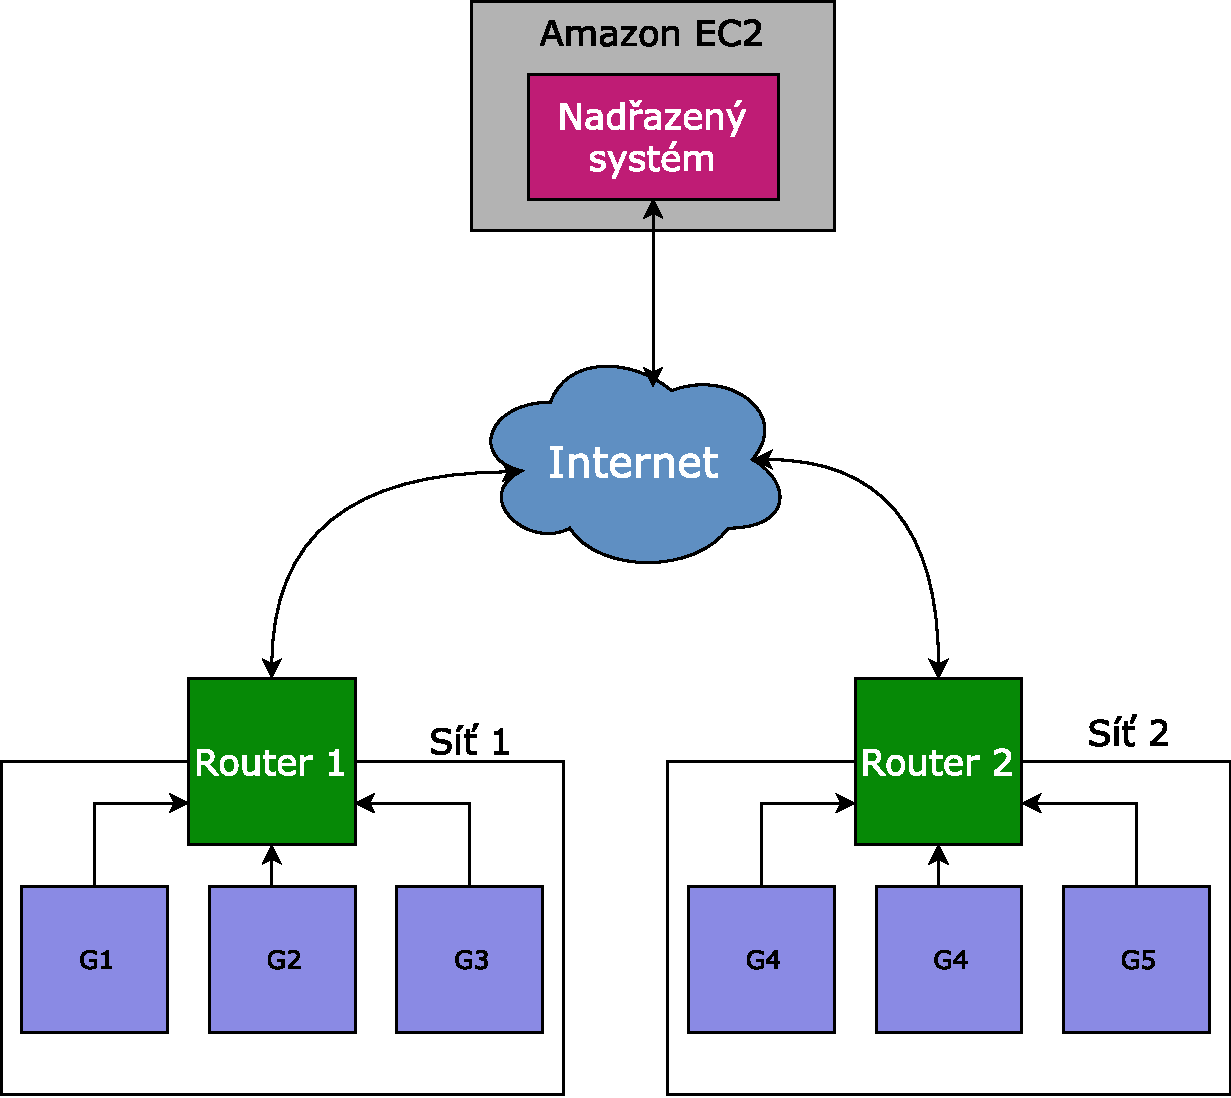
\includegraphics[width=\textwidth]{images/aws.pdf}
    \label{fig:aws}
    \caption[Struktura systému provozovaného na virtuálním serveru]{Struktura systému provozovaného na virtuálním serveru. Podřízené systémy nezasílají požadavky lokálnímu nadřazenému systému v~místní síti, ale globálnímu nadřazenému systému, který je veřejně přístupný na internetu.}
\end{figure}
\chapter{Návrh}
\label{sec:de}

Tato kapitola se zabývá návrhem nadřazeného systému na základě předchozí analýzy z~kapitoly \ref{sec:an}. Nadřazený systém je navržen podle vzoru MVC, jehož jednotlivé části jsou popsány v~sekcích \ref{sec:de_model}, \ref{sec:de_view} a \ref{sec:de_controller}.

Poslední sekce \ref{sec:de_auth} se zabývá návrhem autentizace uživatele při přihlašování do webového rozhraní nadřazeného systému.
 
\section{Návrhový vzor MVC}
\label{sec:de_mvc}

Struktura nadřazeného systému je vhodná k~použití návrhového vzoru MVC, tedy \textit{model-view-controller}. \textit{Model} zde představují garáže (podřízené systémy), k~nim vázané události a logika jejich vyhodnocování. 

\textit{View} je zobrazení těchto dat, tedy především generované HTML stránky webového rozhraní. Jako další \textit{view} je možné považovat získávání dat (například ve formátu JSON) pomocí API nadřazeného systému, třeba při zasílání registračních klíčů podřízeným systémům.

\textit{Controller} je pak část aplikace, která se stará o~zpracování HTTP požadavků. Ty mohou přicházet jednak z~uživateloval prohlížeče, jednak od podřízených systémů. Na základě těchto požadavků pak \textit{controller} posílá příslušné příkazy \textit{modelu}. Struktura aplikace při použití vzoru MVC je naznačena na obrázku \ref{fig:mvc}.

\begin{figure}[h!]
    \centering
    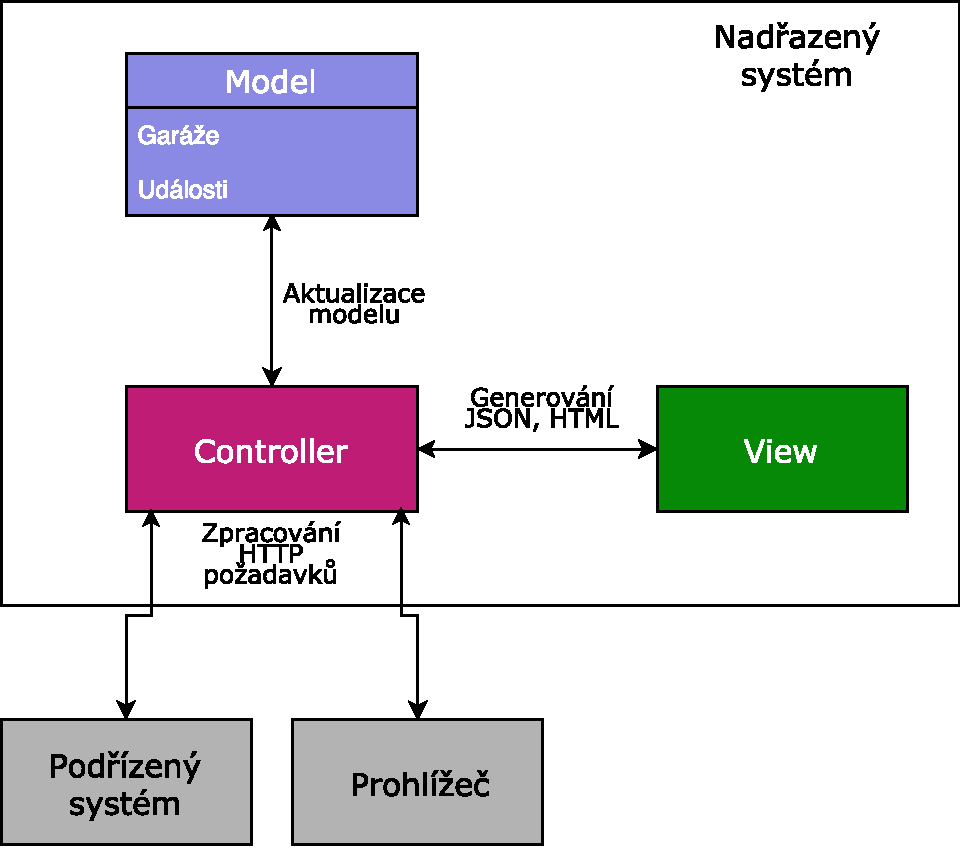
\includegraphics[width=\textwidth]{images/mvc.pdf}
    \caption[Struktura MVC aplikace]{Struktura MVC aplikcace. Uživatel i podřízený systém používají aplikaci pomocí \textit{controlleru}. Ten definuje příslušná URL a zpracovává požadavky na ně -- aktualizuje \textit{model}, případně doručí odpovídající \textit{view}}
    \label{fig:mvc}
\end{figure}

Hlavní motivací pro použití tohoto vzoru je snadná rozšiřitelnost. Pokud by například bylo potřeba aplikaci doplnit o~komunikaci s~podřízenými systémy pomocí MQTT, stačí pouze vytvořit vhodný \textit{controller}. Ten pak může využívat \textit{model} aplikace stejným způsobem jako HTTP \textit{controller}.

Tento návrhový vzor popisuje pouze nadřazený systém spravující garáže. Kromě toho je součástí aplikace ještě autentizace uživatele při přístupu do uživatelského rozhraní. Tuto funkci jsem se rozhodl pojmout jako samostatnou komponentu, popsanou v~sekci \ref{sec:de_auth}.

\section{\textit{Model}}
\label{sec:de_model}

\textit{Model} představuje jádro nadřazeného systému. Je zde implementována vnitřní reprezentace uchovávaných dat, což jsou především zaznamenané události. Každá událost má také svého původce, tedy garáž (přesněji podřízený systém v~této garáži).

Kromě toho \textit{model} implementuje \textit{business logiku} sytému, jako je například vytváření nových garáží (registraci podřízených systémů) či reakce na příchozích události.

Ostatní části aplikace (\textit{view} a \textit{controller}) používají \textit{model}, bez znalosti jeho vnitřní struktury, pomocí následujících operací:

\begin{itemize}
    \item \textbf{Vytvoření garáže} -- registrace nového podřízeného systému. V~případě vytváření pomocí API (tj. přímo podřízeným systémem) vyžaduje operace zapnutý registrační mód. Pokud je nová garáž vytvářena ve webovém rozhraní, zapnutý registrační mód není vyžadován.
    \item \textbf{Editace garáže} -- například změna označení.
    \item \textbf{Smazání garáže} -- smazáním garáže dojde k~odstranění zaznamenaných událostí a zneplatnění příslušného API klíče.
    \item \textbf{Zneplatnění API klíče} -- odepření přístupu podřízenému systému bez nutnosti smazání garáže a s~ní spojených událostí.
    \item \textbf{Zapínání registračního módu} -- v~tomto módu je možné vytvářet nové garáže na základě požadavku od podřízeného systému. Bližší informace jsou v~sekci \ref{sec:de_add_garage}. Registrační mód se po uplynutí časového limitu sám vypne.
    \item \textbf{Přístup k~uloženým datům} -- obecně operace typu získání všech garáží nebo všech událostí vázané ke konkrétní garáži.
    \item \textbf{Vytvoření události} -- základní požadavek využívaný podřízenými systémy.
\end{itemize}

Vnitřně pak model na základě těchto operací autentizuje pomocí API klíčů požadavky podřízených systému, validuje zaslaná data, spravuje databázi nadřazeného systému nebo obstarává zasílání notifikačních e-mailů.

\subsection{Garáž -- \texttt{Garage}}

Třída \texttt{Garage} reprezentuje konkrétní podřízený systém a uchovává s~ním spojená data:

\begin{itemize}
    \item \texttt{id} -- identifikace entity v~databázi.
    \item \texttt{tag} -- uživatelem zvolené označení garáže. To slouží pro snadnější orientaci ve webovém rozhraní (uživatel nemusí garáže rozlišovat podle nic neříkajícího \texttt{id}).
    \item \texttt{note} -- poznámka pro další popis garáže.
    \item \texttt{api\_key} -- klíč umožňující přístup k~API systému. Ten je také zaslán zařízení při jeho registraci. Generování a správa klíčů je blíže popsána v~sekci \ref{sec:de_apikeys}.
    \item \texttt{last\_report} -- datum a čas posledního kontrolního hlášeí.
    \item \texttt{next\_report} -- datum a čas dalšího očekávaného hlášení.
    \item \texttt{period} -- perioda kontrolních hlášení.
    \item \texttt{doors} -- stav dveří garáže (otevřeno/zavřeno).
    \item \texttt{state} -- celkový stav garáže (v~pořádku, nehlásí se atd.).
    \item Seznam událostí spojených s~touto garáží.
\end{itemize}

\subsubsection{Vytváření nových garáží}
\label{sec:de_add_garage}

Nové garáže mohou v~systému vznikat dvěma způsoby. První možnost je vytvoření nové garáže přímo v~uživatelském rozhraní. Po vytvoření se zde zobrazí vygenerovaný API klíč, který je potřeba nahrát na příslušný podřízený systém. Způsob nahrávání by závisel na příslušném hardwaru (například sériová linka). Tato možnost je určena především pro podřízené systémy, které by nepodporovaly zaslání registračního požadavku a nevyžaduje zapnutý registrační mód.

Druhá možnost je použít registrační mód. V~tom případě je nová garáž vytvořena na základě registračního požadavku podřízeného systému (pro bližší informace o~tomto požadavku viz sekci \ref{sec:de_api}). Vygenerovaný API klíč je při tom zaslán jako odpověď na požadavek, a není tedy nutné ho ručně nahrávat. Registrační mód je možné aktivovat v~uživatelském rozhraní. Pokud mód není aktivovaný, nadřazený systém odmítne všechny požadavky na registraci zaslané tímto způsobem.

\subsubsection{API klíče}
\label{sec:de_apikeys}

Podřízené systému se při zasílání událostí přes API prokazují klíčem. Ten slouží jednak k~zamezení příjmu událostí od neautorizovaných systému, jednak k~identifikaci původu události (zdrojové garáže) v~rámci nadřazeného systému. Podřízený systém tedy nemusí znát \texttt{id} garáže, ale jen \texttt{api\_key}.

%generovani klice
Vzhledem k~těmto požadavkům nelze použít jeden univerzální, ale je nutné pro každý registrovaný podřízený systém vygenerovat unikátní klíč. Ten je pak spolu s~dalšími záznamy o~garáži uložen v~databázi systému. K~vytváření klíčů jsem se rozhodl použít systém UUID, umožňující generování náhodných klíčů délky 128 bitů, které jsou (pro praktické účely) unikátní \cite{rfc4122}.

Klíče je možné v~uživatelském rozhraní zneplatnit, a tím odepřít přístup zvolenému podřízenému systému. Tuto operaci lze provést dvěma způsoby. V~prvním případě lze smazat z~databáze celý záznam příslušné garáže. Tím dojde k~zneplatnění jejího klíče, ale také k~odstranění zaznamenaných událostí.

Pokud si uživatel přeje data o~událostech uchovat, může pouze vygenerovat nový API klíč. Přepsáním klíče se opět zneplatní přístup podřízeného systému (který má stále starý klíč), ale uchovají se zaznamenaná data. 

Nově vygenerovaný klíč pak uživatel může nahrát na jiný podřízený systém, a tím například nahradit odcizené monitorovací zařízení. V~tomto případě nelze pro nahrání klíče použít registrační mód nadřazeného systému. Ten totiž vždy počítá s~vytvořením nové garáže.

Vygenerované klíče jsou v~databázi uloženy v~čitelné podobě. Klíče by bylo možné před uložením \textit{hashovat}, čímž by při úniku databáze nedošlo k~jejich prozrazení. V~tom případě by byl klíč v~čitelné podobě v~uživatelském rozhraní zobrazen pouze jednou, při vytvoření nové garáže. Dále už by byl uchováván jeho \textit{hash}.

Pro ukládání klíčů v~čitelné podobě jsem se rozhodl především z~důvodů snadného ladění při implementaci nadřazeného a podřízených systémů. Funkci \textit{hashování} klíčů by v~případě potřeby neměl být problém doplnit.

\subsection{Událost -- \texttt{Event}}
\label{sec:de_event}

Třída \texttt{Event} představuje událost zaznamenanou podřízeným systémem. Jak bylo zmíněno v~sekci \ref{sec:de_mvc}, jsou tyto události vázány ke konkrétním garážím, kdy každá událost má jednoznačně určeného původce, a každá garáž libovolné množství událostí.

Nadřazený systém rozlišuje dva základní druhy událostí. Kontrolní (plánované) události slouží ke kontrole funkčnosti podřízených systémů. Tyto události jsou odesílány v~pravidelném intervalu, určeném nadřazeným systémem. Ten v~odpovědi na požadavek s~kontrolní událostí zašle očekávaný čas (počet minut) do dalšího hlášení.

Kromě kontrolních hlášení mohou podřízené systémy vytvářet mimořádné události. Mimořádná událost nastane při překročení mezních hodnot některého z~čidel (tedy detekce kouře, pohybu či otevření/zavření dveří).

Třída \texttt{Event} obsahuje tyto údaje:

\begin{itemize}
    \item \texttt{id} -- identifikace entity v~databázi.
    \item \texttt{timestamp} -- časové razítko.
    \item \texttt{type} -- typ zaznamenané události. Nadřazený systém rozeznává následující typy:
    \begin{itemize}
        \item \texttt{report} -- kontrolní hlášení.
        \item \texttt{door\_open} -- otevření dveří.
        \item \texttt{door\_close} -- zavření dveří.
        \item \texttt{movement} -- detekce pohybu.
        \item \texttt{smoke} -- detekce kouře.
    \end{itemize}
    \item Garáž, která je původcem události.
\end{itemize}

\subsubsection{Vyhodnocení události}

\begin{figure}[h!]
    \centering
    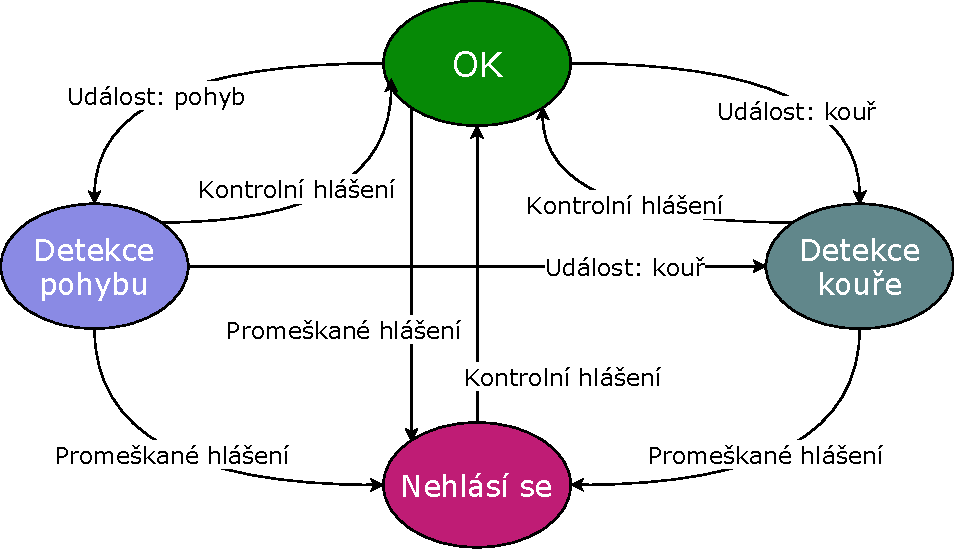
\includegraphics[width=\textwidth]{images/garage_state.pdf}
    \caption[Diagram vyhodnocování stavu garáže]{Diagram vyhodnocování stavu garáže. Nadřazený systém reaguje na příchozí události odpovídající změnou stavu garáže. Změna stavu může být také vyvolána při pravidelné kontrole propásnutých hlášení (přechod do stavu \uv{Nehlásí se})}
    \label{fig:garage_state}
\end{figure}

Příchozí události a stav garáže jsou nadřazeným systémem vyhodnocovány na základě diagramu na obrázku \ref{fig:garage_state}. Změna stavu nastává buď v~reakci na příchozí událost (například detekci kouře) nebo při pravidelné kontrole zaslaných hlášení. 

Pokud při této kontrole nadřazený systém zjistí, že neobdržel očekávané kontrolní hlášení, změní stav garáže na \textcolor{magenta}{\uv{Nehlásí se}}. Tato změna nastane vždy, bez ohledu na předchozí stav. Ze stavu \textcolor{magenta}{\uv{Nehlásí se}} se lze dostat pouze zasláním kontrolního hlášení.

Kontrolní hlášení funguje jako potvrzení, že jakákoliv nenadálá situace v~garáži byla vyřešena. Pokud například podřízený systém detekuje kouř, odešle příslušnou událost a pozdrží další kontrolní hlášení až do doby, kdy bude zdroj kouře odstraněn. Poté může zasláním kontrolního hlášení změnit stav garáže zpět na \textcolor{green}{\uv{OK}}.

Kromě událostí měnících stav garáže nadřazený systém ještě rozeznává události otevření a zavření dveří garáže. Tyto události nemění stav garáže, pouze aktualizují stav dveří. Nejsou tedy součástí tohoto vyhodnocování.

\subsubsection{Zasílání upozornění}

Na základě příchozích událostí odesílá nadřazený systém notifikační e-maily na adresu zvolenou uživatelem. E-mail s~příslušnou událostí je odeslán vždy při změně stavu garáže (mimo změny do stavu \uv{OK}). Tím je zamezeno zbytečnému zasílání duplicitních e-mailů.

%tady pak asi bude i jak to bude celkove s tema mailama

%taky popsat jaky sou moznosti autorizace na tim gmailu (proste smtp meno heslo a pak ty oauth veci) a ze nic z toho neni pro nas uplne idealni

%vidim to bud teda ze tam bude proste smtp klient a holt meno (pak ta emailova schranka muze bejt vicemene jakakoliv, to je taky trochu vyhoda -- tj si uzivatel zalozi stranku treba na seznamu, vyplni meno a heslo a ma to hotovy) a heslo a nebo pouzit nakou sluzbu na posilani mailu. Ten google ma tu oauth autorizaci hrozne slozitou, by asi bylo lepsi neco jako https://github.com/sendgrid/sendgrid-python (https://sendgrid.com/), tam staci proste api klic 

\section{\textit{View}}
\label{sec:de_view}

Hlavním \textit{view} nadřazeného systému je webové uživatelské rozhraní. Zde se zobrazuje celkový stav systému, jednotlivých garáží, a zachycené události. Také jsou ze přístupné ovládací prvky pro správu systému. Návrhem tohoto rozhraní se zabývá následující sekce \ref{sec:de_web}.

Další \textit{view} aplikace představují odpovědi (například vygenerované API klíče) nadřazeného systému podřízeným systému při zpracování jejich požadavků. Tento \textit{view} je popsán společně s~API systému v~sekci \ref{sec:de_api}.

\subsection{Webové rozhraní}
\label{sec:de_web}

Webové rozhraní představuje prostředí umožňující uživatel správu celého nadřazeného systému. Rozhraní tvoří hlavní stránka, stránky jednotlivých garáží a stránky uživatelského nastavení (změna hesla a nastavení notifikací).

Případy užití rozhraní se dají shrnout do tří kategorií, popsaných na obrázku \ref{fig:use_case_top}.

\begin{figure}[h!]
    \centering
    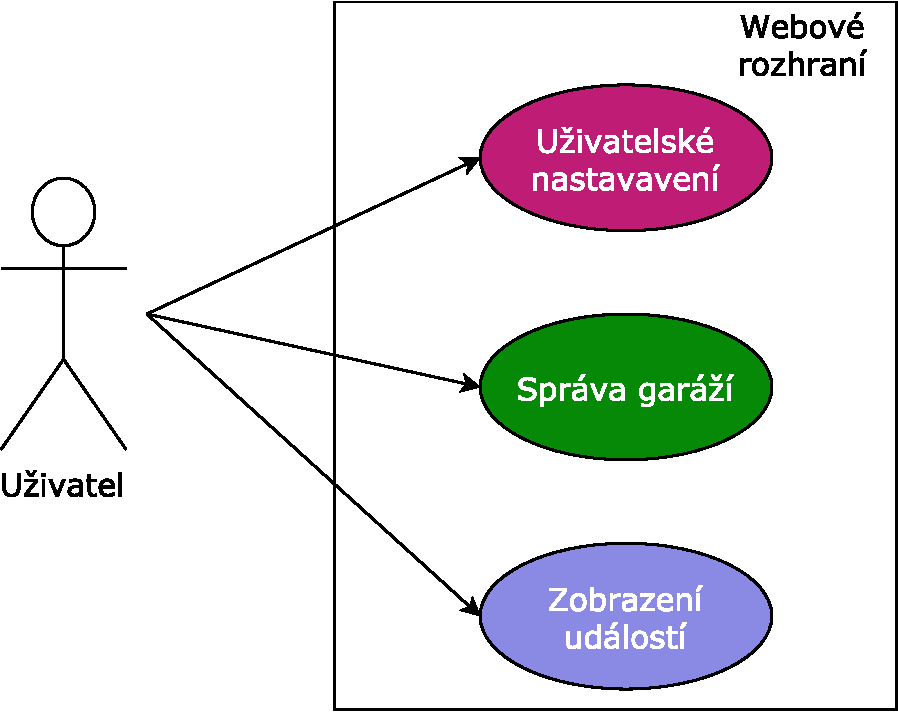
\includegraphics[width=0.9\textwidth]{images/use_case_top.pdf}
    \caption[Vrchní úroveň případů užití webového rozhraní]{Vrchní úroveň případů užití webového rozhraní. Uživatel do aplikace přistupuje buď za účelem změny uživatelského nastavení, správy jednotlivý podřízených systémů, případně kvůli kontrole zaznamenaných událostí}
    \label{fig:use_case_top}
\end{figure}

\subsubsection{Správa garáží}

Správu garáží tvoří případy užití popsané na obrázku \ref{fig:use_case_garage}. Operace vytvoření garáže a zapnutí registračního módu nejsou vázané k~žádné konkrétní garáži, a jsou tedy k~dispozici na hlavní stránce webového rozhraní ihned po přihlášení. 

Na hlavní stránce je také zobrazen seznam všech sledovaných garáží včetně jejich stavu, posledního hlášení, dalšího plánovaného hlášení a odkazu na stránku garáže, která obsahuje zbylé možnosti, vázané ke konkrétní garáži.

\begin{figure}[h!]
    \centering
    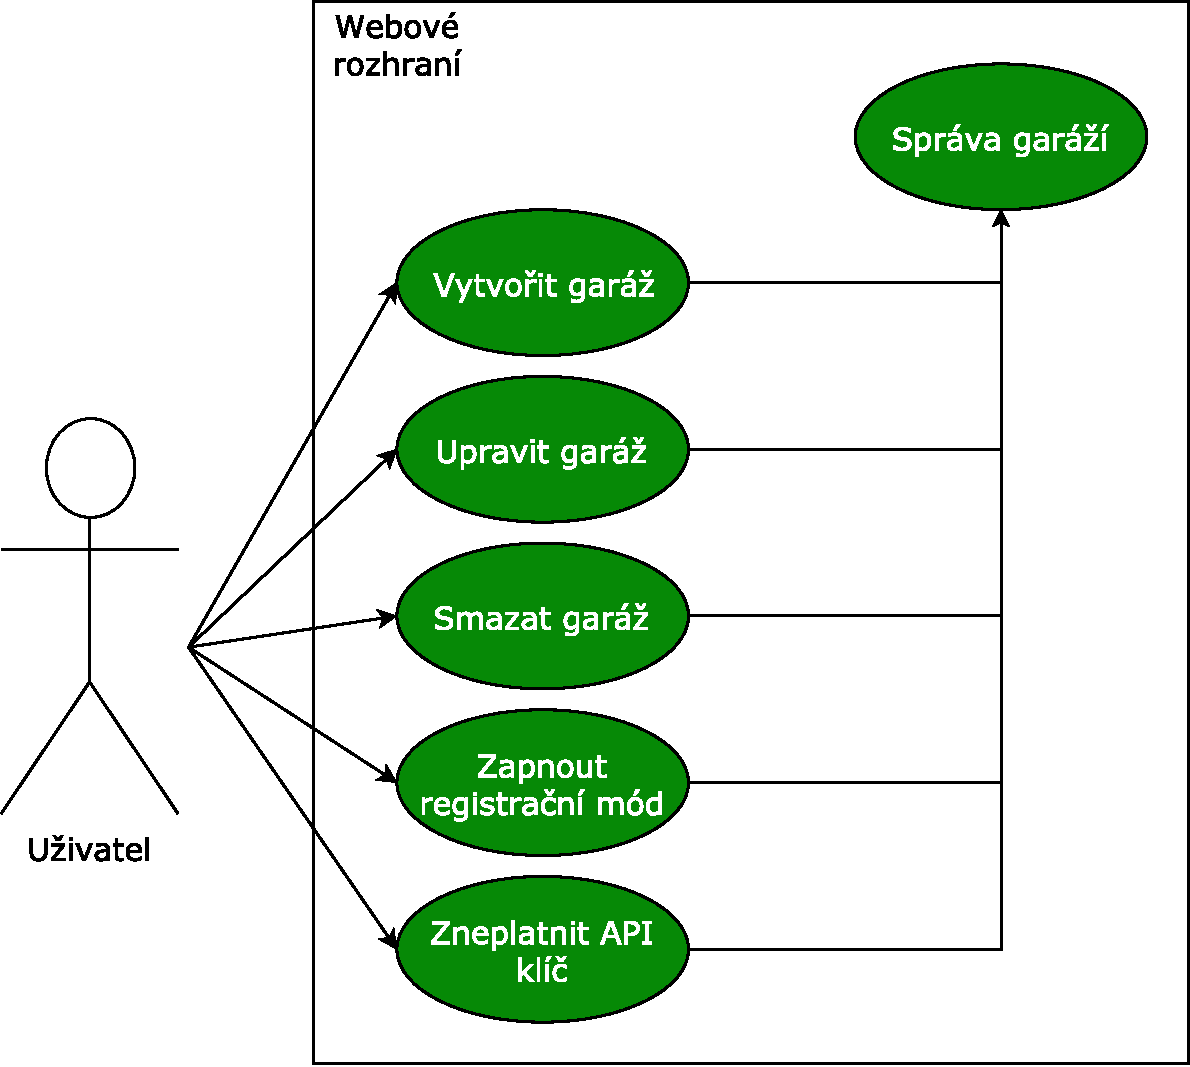
\includegraphics[width=\textwidth]{images/use_case_garage.pdf}
    \caption[Případy užití správy garáží]{Případy užití správy garáží. Zde uživatel zobrazuje stav garáží a jednotlivé garáže spravuje pomocí uvedených operací}
    \label{fig:use_case_garage}
\end{figure}

\subsubsection{Zobrazení událostí}

Případy užití z~kategorie zobrazení událostí popisuje obrázek \ref{fig:use_case_events}. Na stránce garáže může uživatel zobrazit s~ní spojené události. Seznam událostí pak může filtrovat podle typu (viz sekci \ref{sec:de_event}).

\begin{figure}[h!]
    \centering
    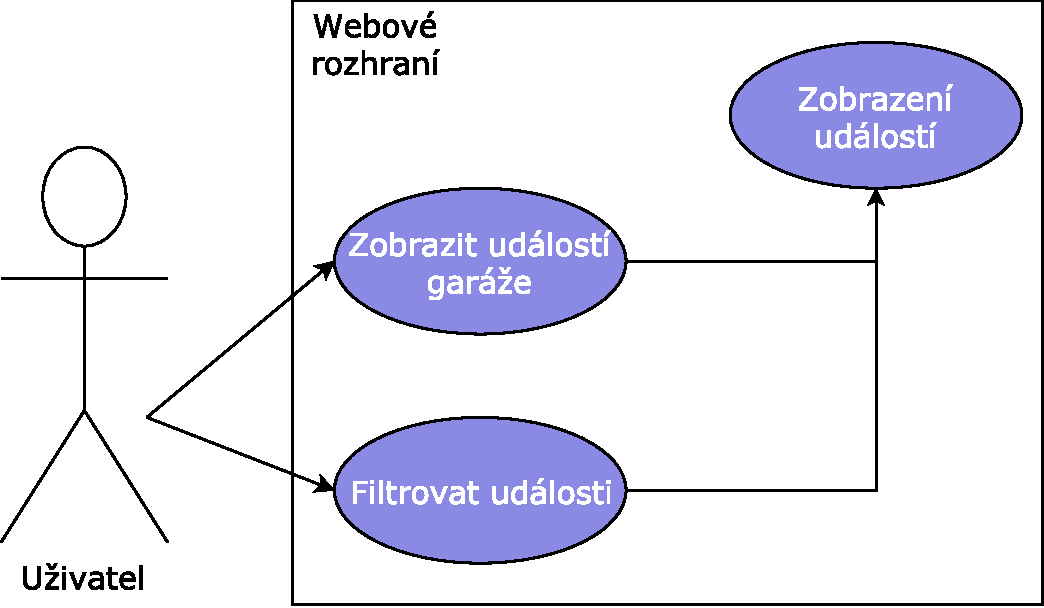
\includegraphics[width=\textwidth]{images/use_case_events.pdf}
    \caption[Případy užití zobrazení událostí]{Případy užití zobrazení událostí. Uživatel zobrazuje události spojené s~konkrétní garáží. Zobrazené událostí filtruje podle jejich typu}
    \label{fig:use_case_events}
\end{figure}

\subsubsection{Uživatelské nastavení}
\label{sec:de_user_settings}

%tady este neco bude ofc

Uživatelské nastavení není uloženo přímo v~databázi, ale zvlášť v~konfiguračním souboru \texttt{user\_settings.ini}. Díky tomu je snazší toto nastavení v~případě potřeby změnit i bez nutnosti otvírat webové rozhraní.

\begin{figure}[h!]
    \centering
    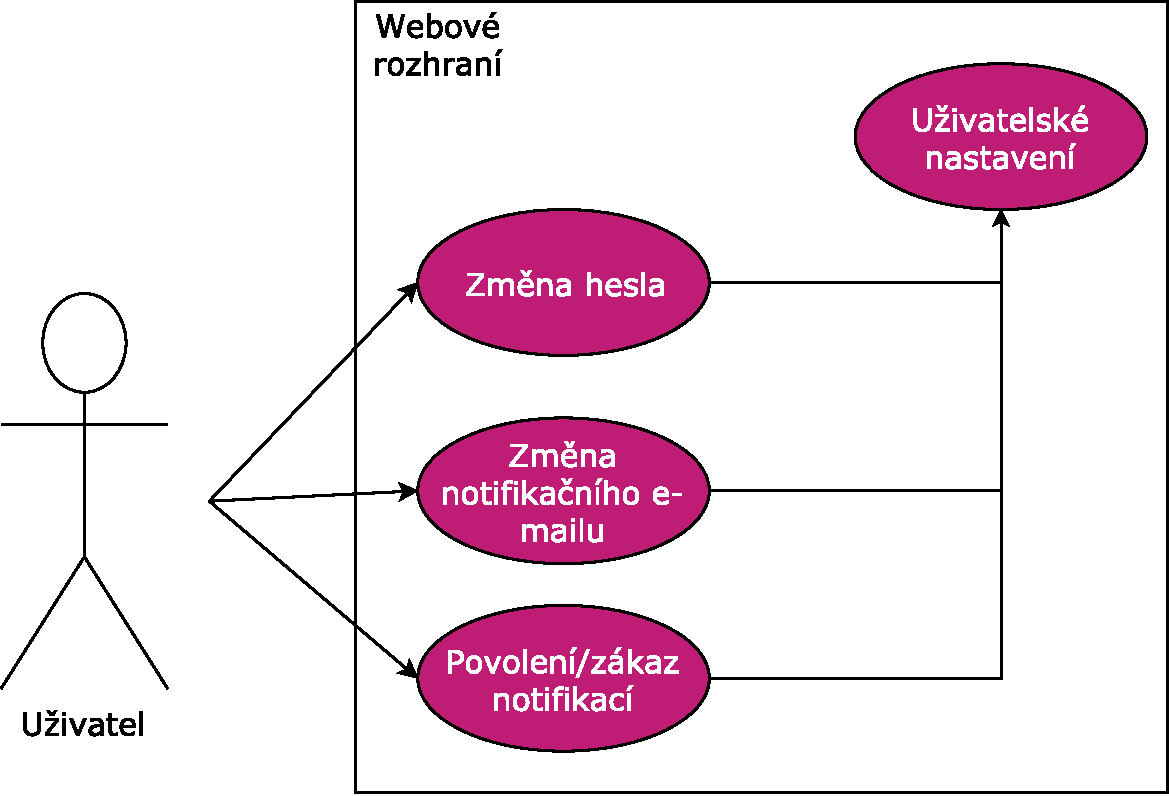
\includegraphics[width=\textwidth]{images/use_case_user.pdf}
    \caption[Případy užití uživatelského nastavení]{Případy užití uživatelského nastavení. Uživatel ve webovém rozhraní provádí změnu hesla, změnu notifikačního e-mailu, případně zákaz/povolení notifikací}
    \label{fig:use_case_user}
\end{figure}


\section{\textit{Controller}}
\label{sec:de_controller}

\textit{Controller} slouží ke zpracování požadavků uživatele a podřízených systémů. Jelikož jde o~HTTP požadavky, definuje \textit{controller} URL, přiřazuje k~nim akce, které se mají provést (kontrola přihlášení, přesměrování atd.) a vrací příslušné odpovědi (například vygenerované stránky).

\textit{Controller} aplikace se dá rozdělit na dvě části. První část zpracovává požadavky zaslané uživatelem z~webového rozhraní. Propojuje tedy případy užití popsané v~sekci \ref{sec:de_web} s~operacemi na modelu ze sekce \ref{sec:de_model}. URL definovaná v~této části jsou využívána pouze uvnitř aplikace, a nejsou součástí API nadřazeného systému.

Druhá část zpracovává požadavky podřízených systémů. Zde definovaná URL tvouří API nadřazeného systému, pomocí kterého se mohou podřízené systémy registrovat a nahrávat nové události. Popisem API, včetně formátu požadavků a návratových hodnot, se zabývá sekce \ref{sec:de_api}.

\subsection{API}
\label{sec:de_api}

%https://docs.microsoft.com/en-us/azure/architecture/best-practices/api-design

API nadřazeného systému slouží ke komunikaci s~podřízenými systémy. S~jeho pomocí se podřízený systém může registrovat a začít nadřazenému systému posílat zaznamenané události.

Odpovědi nadřazeného systému na příchozí požadavky jsou ve formátu JSON. Každá odpověď obsahuje návratový kód a případně další data, která je nutné zaslat podřízenému systému.

\subsubsection{Registrační požadavek}

Registrační požadavek slouží k~zaregistrování nového podřízeného systému a vytvoření záznamu s~ním spojené garáže. Hlavním účelem tohoto požadavku je snadná distribuce API klíče na podřízené systémy -- klíč není nutné nahrávat ručně, ale je odeslán v~odpovědi na tento požadavek (pro bližší informace o~klíčích viz sekci \ref{sec:de_apikeys}).

Kvůli bezpečnosti je tento požadavek povolen pouze pokud je v~uživatelském rozhraní zapnutný registrační mód. Pokud je mód vypnutý, odpovídá nadřazený systém na všechny registrační požadavky chybovým kódem \textit{403 -- Forbidden}. Tím je částečně zabráněno registraci nežádoucích podřízených systémů.

Registrační požadavek má následující formát (zaslání registračního požadavku v~jazycke Python je popsáno v~ukázce \ref{lst:api_reg}):

\begin{itemize}
    \item URL -- \texttt{/api/garages}.
    \item HTTP metoda -- POST.
    \item Návratová hodnota -- JSON:
    \begin{itemize}
        \item \texttt{status} -- návratový kód (201 při vytvoření garáže, 403 při vypnutém reg. módu).
        \item \texttt{api\_key} -- unikátní klíč k~API nadřazeného systému (pouze v~případě úspěchu, tedy vytvoření garáže).
    \end{itemize}
\end{itemize}

\begin{listing}[htbp]
\caption{\label{lst:api_reg} Zaslání registračního požadavku nadřazenému systému provozovaném na adrese \texttt{raspberrypi.local}}
\begin{minted}[bgcolor=codebg]{python}
import requests
# server nadrazeneho systemu je pristupny
# na adrese raspberrypi.local
url = 'https://raspberrypi.local/api/garages'

# pozadavek 'post', bez overeni
# self-signed certifikatu
r = requests.post(url, verify=False)

if r.status == 201:
    api_key = r.json()['api_key']
\end{minted}
\end{listing}

\subsubsection{Kontrolní hlášení}

Kontrolní hlášení slouží k~ověření činnosti podřízeného systému. Jeho zasláním podřízený systém také potvrzuje, že stav sledované garáže je v~pořádku. 

Požadavek zasílající kontrolní hlášení má tento formát:

\begin{itemize}
    \item URL -- \texttt{/api/report\_event}.
    \item HTTP metoda -- POST.
    \item Hlavička požadavku:
    \begin{itemize}
        \item \texttt{api\_key} -- unikátní klíč k~API nadřazeného systému.
    \end{itemize}
    \item Návratová hodnota -- JSON:
    \begin{itemize}
        \item \texttt{status} -- návratový kód (201 při vytvoření hlášení, 403 při neplatném klíči).
        \item \texttt{period} -- počet minut do dalšího očekávaného hlášení.
    \end{itemize}
\end{itemize}

\begin{listing}[htbp]
\caption{\label{lst:api_report} Zaslání kontrolního hlášení nadřazenému systému provozovaném na adrese \texttt{raspberrypi.local}}
\begin{minted}[bgcolor=codebg]{python}
import requests
# server nadrazeneho systemu je pristupny
# na adrese raspberrypi.local
url = 'https://raspberrypi.local/api/report_event'

# api klic (ziskany napriklad reg. pozadavkem)
# je zasilan v~hlavicce pozadavku
headers = {'api_key' : api_key}

# pozadavek 'post', bez overeni
# self-signed certifikatu
r = requests.post(url, headers=headers, verify=False)

if r.status == 201:
    #odpoved -- cas do dalsiho hlaseni
    period = r.json()['period']

\end{minted}
\end{listing}

\subsubsection{Ostatní události}

Vytváření dalších událostí je stejné jako vytváření kontrolního hlášení. Liší se pouze použité URL. Odpovědi na tyto požadavky neobsahují žádná data od nadřazeného systému, pouze návratový kód informující o~úspěchu či chybě:

\begin{itemize}
    \item URL -- podle typu události:
    \begin{itemize}
        \item \texttt{/api/door\_open\_event}
        \item \texttt{/api/door\_close\_event}
        \item \texttt{/api/movement\_event}
        \item \texttt{/api/smoke\_event}
    \end{itemize}
    \item HTTP metoda -- POST.
    \item Hlavička požadavku:
    \begin{itemize}
        \item \texttt{api\_key} -- unikátní klíč k~API nadřazeného systému.
    \end{itemize}
    \item Návratová hodnota -- JSON:
    \begin{itemize}
        \item \texttt{status} -- návratový kód (201 při vytvoření události, 403 při neplatném klíči).
    \end{itemize}
\end{itemize}

\begin{listing}[htbp]
\caption{\label{lst:api_report} Zaslání události detekce kouře nadřazenému systému provozovaném na adrese \texttt{raspberrypi.local}}
\begin{minted}[bgcolor=codebg]{python}
import requests

# stejne jako pri zasilani kontrolniho hlaseni
# lisi se pouze url
url = 'https://raspberrypi.local/api/smoke_event'
headers = {'api_key' : api_key}

r = requests.post(url, headers=headers, verify=False)

if r.status == 201:
    #odpoved neobsahuje zadna data
    ...

\end{minted}
\end{listing}

\section{Autentizace uživatele}
\label{sec:de_auth}

Do webového rozhraní aplikace je povolen pouze autorizovaný přístup, a je tedy nutné nějakým způsobem ověřit identitu uživatele. Jelikož aplikace nepočítá s~odlišnými stupni přístupu (a tedy každý uživatel s~přístupem do rozhraní má přístup ke všem jeho částem), rozhodl jsem se, že nebudu vytvářet infrastrukturu uživatelských účtů, protože by měla pouze omezené využití.

Přístup do rozhraní tedy nevyžaduje vytvoření účtu a zadávání uživatelského jména, ale pouze heslo. \textit{Hash} tohoto hesla (doplněného solí), vytvořený pomocí algoritmu Bcrypt, je uložen v~souboru s~uživatelským nastavením aplikace.

\textit{Hashování} hesla je zde použito především pro případ, že by uživatel použil stejné heslo jaké používá v~jiných aplikacích či službách. V~případě prozrazení uživatelských dat (například při odcizení systému) tedy útočník nemůže z~otisku zjistit původní použité heslo, tudíž přístup k~těmto uživatelovým účtům není kompromitován.

Stejně tak někdo s~přístupem k~serveru, na kterém nadřazený systém běží, nemá automaticky přístup do webového rozhraní. Nicméně má stále přístup k~celé (nešifrované) databázi a také může heslo libovolně měnit (spočítáním nového otisku), tedy z~praktického hlediska je přístup k~serveru téměř ekvivalentní s~přístupem do webového rozhraní.

\subsection{První přihlášení}

Při prvním startu nadřazeného systému je zvoleno jednoduché implicitní heslo (\textit{password}), kterým se uživatel může přihlásit do webového rozhraní. 

Pokud nadřazený systém detekuje použití tohoto hesla, po přihášení uživatele ihned přesměruje na stránku umožňující změnu hesla a zobrazí příslušné varování.
\chapter{Implementace}
\label{sec:im}

V~této kapitole je popsána implementace nadřazeného systému podle návrhu z~kapitoly \ref{sec:de}. Jednotlivé sekce tedy popisují implementační detaily dílčích částí návrhového vzoru MVC. Poslední sekce \ref{sec:im_auth} se zabývá implementací autentizace uživatele.

\section{Struktura aplikace}

Aplikace nadřazeného systému je rozdělena do tří modulů:

\begin{itemize}
    \item \texttt{mod\_main} -- hlavní modul aplikace. V~tomto modulu je implementován \textit{model} systému popsaný v~sekci \ref{sec:de_model}. \textit{Model} je využíván i ostatními moduly (konkrétně modulem \texttt{mod\_api}). Dále tento modul implementuje webové rozhraní správy nadřazeného systému.
    \item \texttt{mod\_api} -- modul implementující API systému. Zde je implementována část \textit{controlleru} ze sekce \ref{sec:de_api}, definující URL, pomocí kterých mohou podřízené systémy komunikovat s~nadřazeným systémem.
    \item \texttt{mod\_auth} -- modul implementující autentizaci uživatele při přihlašování do webového rozhraní.
\end{itemize}

K~rozdělení aplikace na jednotlivé moduly je použit nástroj frameworku Flask nazvaný \textit{blueprints} \cite{flask_blueprints}.  Hlavní důvod k~využití modulů je oddělení částí aplikace podle jejich funkce.

Při strukturování aplikace jsem vycházel z~článku \textit{How To Structure Large Flask Applications} \cite{flask_large}.

\section{Implementace \textit{modelu}}

Jak je zmíněno v~sekci \ref{sec:de_model}, \textit{model} aplikace je tvořen třídami \texttt{Garage} a \texttt{Event}. Tyto třídy přímo využívají databázi nadřazeného systému, k~jejich implementaci je proto použit framework SQLAlchemy \cite{sqlalchemy}, který výrazně usnadní práci s~databází.

Tento framework poskytuje přístup k~SQL databázím přímo z~jazyka Python, takže není nutné psát prakticky žádný SQL kód. Tabulku v~databázi je možné definovat jako Python třídu s~přísušnými atributy a SQLAlchemy vytvoří odpovídající databázové schéma. 

SQLAlchemy také umožňuje snadno definovat databázové vztahy. V~\textit{modelu} nadřazeného systému se vyskytuje pouze vztah $1:N$ mezi třídami \texttt{Garage} a \texttt{Event} (jedna garáž má mnoho událostí, každá událost má právě jednu garáž). Tento vztah je pomocí SQLAlchemy definován následujícím způsobem:

\begin{listing}[htbp]
\caption{\label{lst:db_relationship} Vytvoření vztahu $1:N$ mezi třídami \texttt{Garage} a \texttt{Event}}
\begin{minted}[bgcolor=codebg]{python}
from sqlalchemy import Column, ForeignKey, Integer
from sqlalchemy.ext.declarative import declarative_base
from sqlalchemy.orm import relationship

Base = declarative_base()

# třídy Event a Garage
# dědí SQLAlchemy metody
# třídy Base
class Event(Base):
    ...
    # odkaz na příslušnou garáž
    garage_id = Column(Integer, ForeignKey(
        'Garage.id'), nullable=False)

class Garage(Base): 
    ...
    # definice 1:N vztahu mezi garáží a událostí
    events = relationship('Event', backref='Garage')
\end{minted}
\end{listing}

\subsection{Kontrola zmeškaných hlášení}

V~databázi nadřazeného systému je potřeba pravidelně provádět kontrolu, zda podřízené systémy zaslaly v~očekávaný čas kontrolní hlášení. Pokud bylo plánované hlášení promeškáno, je nutné změnit stav příslušné garáže na \uv{Nehlásí se}.

Aplikace nadřazeného systému nemá v~zásadě možnost, jak tuto kontrolu sama iniciovat, neboť pouze reaguje na příchozí požadavky (od uživatele či podřízeného systému). Provedení kontroly může být důsledkem takového požadavku, například pokud uživatel otevře hlavní stránku webového rozhraní. 

Provádět kontrolu hlášení pouze v~reakci na vnější podnět však není dostatečné. Pokud by nadřazený systém musel pro provedení kontroly hlášení čekat interakci s~webovým rozhraním (nebo například s~podřízeným systémem), nemuselo by vůbec dojít ke změně stavu garáže a tedy ani k~odeslání notifikačního e-mailu. Je tedy nutné zajistit pravidelné provádění kontrol na základě vnitřního podnětu.

Tento problém jsem vyřešil použítím plánovače APScheduler \cite{apscheduler}. APScheduler funguje jako knihovna do Pythonu, a umožňuje plánovat provádění zvolených funkcí. Nejde tedy o~externí program, plánovač je přímo součástí kódu nadřazeného systému \cite{apscheduler}. Vytvoření pravidelné kontroly hlášení podřízených systémů je implementováno tímto způsobem:

\begin{listing}[htbp]
\caption{\label{lst:scheduler_check} Pravidelná kontrola hlášení podřízených systémů pomocí knihovny APScheduler. Po startu plánovače je každých 5 minut volána metoda \texttt{Garage.check\_reports()}}
\begin{minted}[bgcolor=codebg]{python}

from apscheduler.schedulers.background import \
    BackgroundScheduler

# BackgroundScheduler běží v~samostatném vlákně,
# neblokuje tedy webovou aplikaci
scheduler = BackgroundScheduler()

# přidání pravidelného úkolu do plánovače
# Garage.check_reports je statická metoda
# třídy Garage, která provede kontrolu hlášení
# u~všech garáží v~databázi (a případně upraví jejich stav)
scheduler.add_job(Garage.check_reports, 'interval', minutes=5)
scheduler.start()
\end{minted}
\end{listing}

Plánovač se kromě kontroly hlášení hodí také při vypínání registračního módu. Ten z~bezpečnostních důvodů po aktivaci běží po dobu tří minut. Jeho vypnutí je naplánováno obdobně jako kontrola hlášení, jediný rozdíl je, že úkol není spouštěn v~pravidelném intervalu, ale pouze jednou.

\subsection{Zasíláním upozornění}

%posilani mailu pomoci toho eventu zmeny v sqlalchemy

%posilani mailu obecne jak je implementovany

\section{Implementace \textit{view}}

Tato část se věnuje implementaci stránek webového rozhraní nadřazenéh systému. Jednotlivé HTML stránky rozhraní jsou generovány pomocí šablonovacího systému Jinja \cite{jinja}, který je součástí frameworku Flask \cite{flask_templates}. 

Jinja umožňuje dynamické generování HTML stránek z~předem vytvořených šablon a dalších vstupnů, v~tomto případě především dat z~\textit{modelu} aplikace. Tato data jsou šabloně předána \textit{controllerem} (viz sekci \ref{sec:im_controller}). V~šablonách Jinja používá syntaxi založenou na Pythonu \cite{jinja}. Například HTML šablona pro tabulku se zaznamenanými událostmi vypadá následovně:

\begin{listing}[htbp]
\caption{\label{lst:jinja_table} HTML šablona tabulky zaznamenaných událostí, využívající šablonovací systém Jinja. Proměnná \texttt{garage} je šabloně předána \textit{controllerem} aplikace}
\begin{minted}[bgcolor=codebg]{html}
<table class=basic_table>
    <tr>
    <th>Seznam událostí</th>
    </tr>
    <!-- použítí cyklu v~systému Jinja -->
    
        <tr>
            <!-- přístup k~proměnné pomocí bloku {{ }} -->
            <td class=event_type_{{event.type}}>
                {{ event | event_filter }}
            </td>
        </tr>
     <!--konec bloku cyklu -->
</table>
\end{minted}
\end{listing}

Jinja také ďovoluje definici filtrů, sloužících ke zpracování zobrazovaných dat \cite{jinja}. V~ukázce \ref{lst:jinja_table} je použit filtr \texttt{event\_filter}. Ten dostane jako vstup instanci třídy \texttt{event} a vytvoří její textovou reprezentaci s~údaji o~typu a času události. Tím je oddělena implementace této třídy v~\textit{modelu} a její zobrazení ve \textit{view}.

\subsection{Formuláře}
\label{sec:im_forms}

Webové rozhraní obsahuje několik formulářů, které slouží například k~editaci garáže či změně hesla. Tyto formuláře jsou implementovány pomocí frameworku WTForms, který je opět integrován ve Flasku \cite{flask_wtf}.

Framework poskytuje třídu \texttt{FlaskForm}, pomocí které je možné vytvořit podtřídy popisující jednotlivé formuláře \cite{flask_wtf}. V~těchto podtřídách jsou pak definovány pole formuláře.

U~některých polí je potřeba provádět kontrolu zadávaných hodnot (například dodržení minimální délky hesla). To je provedeno pomocí další součásti WTForms, nazvané validátory \cite{flask_wtf}. Pomocí těchto předdefinovaných validátorů lze na vstupní data aplikovat nejrůznější omezení (délka řetězce, rozsah číselných hodnot atd.) a určit chybovou zprávu zobrazenou při jejich porušení \cite{flask_wtf}.

Využití tohoto frameworku při implementaci formuláře pro editaci údajů garáže popisuje ukázka \ref{lst:wtform}. Vygenerování HTML kódu formuláře, včetně zobrazení chybových zpráv po odeslání neplatného formuláře, je provedeno pomocí systému Jinja.

\begin{listing}[htbp]
\caption{\label{lst:wtform} Implementace formuláře pro editaci údajů garáže pomocí frameworku WTForms. Při kontrole vstupu je ověřen rozsah zadávané periody}
\begin{minted}[bgcolor=codebg]{python}
from flask_wtf import FlaskForm
from wtforms import StringField, IntegerField, TextAreaField
from wtforms.validators import NumberRange

class GarageForm(FlaskForm):
    tag = StringField('Označení')
    period = IntegerField('Perioda hlášení (minuty)', 
        validators=[
        NumberRange(1, 999, 
            message='Perioda musí být mezi 1 a 999')
        ])
    note = TextAreaField('Poznámka')
\end{minted}
\end{listing}

\subsection{Filtrování událostí}

Při zobrazení seznamu událostí konkrétní garáže je možné tyto události filtrovat podle jejich typu. Filtrování je prováděno na straně klienta (v~prohlížeči) pomocí Javascriptu a knihovny jQuery \cite{jquery_about}.

\section{Implementace \textit{controlleru}}
\label{sec:im_controller}

\textit{Controller} aplikace je implementován spárováním URL a funkce, která se má provést při příchozím požadavku na toto URL. Jako odpověď na požadavek je pak klientovi zaslána návratová hodnota funkce. Tento princip (demonstrovaný v~ukázce \ref{lst:route}) představuje základní stavební kámen při tvorbě \textit{controlleru} ve frameworku Flask.

Pro spárování funkce a URL je použit dekorátor \texttt{route}. Dekorátor je konstrukt jazyka Python, který umožňuje rozšířit danou funkci či metodu o~další funkcionalitu \cite{python_decorators}. Pomocí dekorátoru \texttt{route} je definováno URL a případně i povolené HTTP metody, které může klient při požadavku použít. Implicitně je povolena pouze metoda \texttt{get} \cite{flask_api}. 

\begin{listing}[htbp]
\caption{\label{lst:route} Přiřazení funkce k~URL. Funkce \texttt{index} bude zavolána při každém příchozím požadavku s~metodou \texttt{get} na kořenové URL \texttt{/}. Návratová hodnota funkce je vygenerovaná HTML stránka, která bude zaslána klientovi}
\begin{minted}[bgcolor=codebg]{python}
from flask import Blueprint, render_template

from .models.garage import Garage 

# deklarace blueprintu mod_main
mod_main = Blueprint('main', __name__)

# URL a příslušná akce jsou definovány
# vzhledem k~blueprintu
@mod_main.route('/')
@login_required # kontrola přihlášení uživatele
def index():
    # získání údajů o~všech garážích
    garages = Garage.query.all()

    # vygenerování stránky pomocí Jinja
    # zobrazovaná data jsou předána jako
    # parametry funkce render_template()
    return render_template('main/index.html', 
                            garages=garages, 
                            reg_mode=Garage.reg_mode)
\end{minted}
\end{listing}

Pokud funkce zpracovávající požadavek mění obsah databáze (například vytváří novou garáž), je u~požadavku vyžadována metoda \texttt{post}. Tyto požadavky jsou také chráněny proti CSRF útoku. Do každého formuláře používajícího metodu \texttt{post} je vložen náhodně generovaný \textit{token}, podle kterého může aplikace ověřit původ požadavku. Ochrana proti CSRF je automaticky zapnuta u~všech formulářů vytvořených pomocí WTForms (viz sekci \ref{sec:im_forms}) \cite{flask_wtf}.

%csrf, viz  napsat ze pro add garage a revoke key misto normalni routy, getu a linku pouzivame formulare a post kvuli vochrane pred csrf, viz \url{https://stackoverflow.com/questions/6812765/how-to-demonstrate-a-csrf-attack}. Timhle utokem by nekdo moh vytvaret garaze a rusit api klice, coz neni naka velka skoda ale spis na votravovani no (u~vostatnich veci (tj hlavne change password) to bylo uz driv v~pohode protoze byly pouzity ty flaskforms)

\subsection{Implementace API}

%vyjimka z csrf (neni potreba login, prokazuje se klicem)

Způsobem popsaným v~sekci \ref{sec:im_controller} je implementováno i API nadřazeného systému. Operace a URL ze sekce \ref{sec:de_api} jsou spárovány s~příslušnými funkcemi, upravujícími \textit{model} aplikace.

Jelikož se podřízené systémy prokazují pomocí API klíče, není zde nutné provádět žádnou kontrolu přihlášení jako při zpracování požadavků ve webovém rozhraní. Pouze je zkontrolována přítomnost zaslaného klíče v~databázi. Také není nutné implementovat ochranu proti CSRF útokům.

\section{Autentizace uživatele}
\label{sec:im_auth}

%asi hlavne bcrypt popsat

%login_required decorator \url{http://flask.pocoo.org/docs/0.12/patterns/viewdecorators/}

%session

%pouziti metody post pri posilani login udaju

%mozna csrf tady, napsat jak je tam zapnuty, ze default je soucasti toho flask_formu ale my ho chceme pro vsechny ty post routy a pak vyjimku pro api modul -- tady napsat jak se nam siknou ty blueprinty

%v~testovani je mozny tenhle utok demonstrovat a ukazat jak pekne nam to funguje (voproti ty prvni verzi kde byl na add garage normalne get). Ted se pri tim pokusu vo utok normalne zvobrazi invalid csrf token nebo tak neco. Pro porovnani zmen puvodni a vopraveny verze viz commit e52a54b2caa8eead85e8df28c738356a7541a1c4 (password redirect, to je posledni verze s~timhle bugem)

\chapter{Testování}
\label{sec:te}

%tady napsat nakej strucnej uvod jako je v tech predchozich kapitolach az budem mit tu propustnost

\section{Automatizované testy}

K~aplikaci jsem vytvořil sadu automatizovaných testů, které ověřují funkčnost jednotlivých komponent. Konkrétně jde o~testy pro \textit{model} aplikace (zde je testována především třída \texttt{Garage}), webové rozhraní a API systému. Tyto testy byly implementovány pomocí frameworku pytest \cite{pytest}.

Části aplikace, u~kterých je automatizované testování problematikcé, jako například funkce využívající APScheduler (viz sekci \ref{sec:im_scheduler}) nebo zasílání notifikací, jsem otestoval ručně.

\subsection{Testovací konfigurace}

Před spuštěním automatizovaných testů je nutné upravit konfiguraci aplikace. Především je třeba určit umístění testovací databáze a souboru s~uživatelským nastavením. Tyto soubory jsou v~průběhu testů upravovány a po dokončení smazány.

Také je nutné vypnout ochranu proti CSRF v~celé aplikaci, což výrazně zjednodušší testování formulářů aplikace. Jelikož požadavky s~metodou \texttt{post} vytvořené v~testech nepocházejí z~webových stránek aplikace, nemohou dodat CSRF \textit{token}, který je součástí formuláře. 

Sdílení \textit{tokenu} mezi aplikací a testy by sice bylo možné implementovat, bylo by však zbytečně komplikované. Za vhodnější postup považuji vypnutí CSRF ochrany pro většinu testů a funkčnost ochrany otestovat v~samostatném testu (viz sekci \ref{sec:te_csrf}).

Změna konfigurace aplikace je provadena nastavením proměnné prostředí \texttt{GARAGE\_SYSTEM\_CONFIG} na soubor s~testovací konfigurací (viz sekci \ref{sec:im_config}).

\subsection{Testování \textit{modelu}}
\label{sec:te_model}

Testování \textit{modelu} aplikace spočívá především v~testování metod třídy \texttt{Garage}. Třída \texttt{Event} slouží pouze k~uchování dat o~události a neimplementuje žádné metody, které by bylo možné testovat.

Testovány jsou následující scénáře:

\begin{itemize}
    \item Přidání garáže.
    \item Smazání garáže.
    \item Kontrola zmeškaných hlášení.
    \item Zaslání kontrolního hlášení.
    \item Změna stavu po zaslání události.
    \item Zneplatnění API klíče.
    \item Získání zaznamenaých událostí podle typu.
\end{itemize}

Zde stojí za zmínku test kontroly zmeškaných hlášení. V~něm je garáži zasláno kontrolní hlášení, čímž je určen čas dalšího očekávaného hlášení. Po překročení tohoto času je potřeba otestovat, zda byl stav garáže změnen na \uv{Nehlásí se}.

Jelikož je minimální perioda hlášení 1 minuta, prosté čekání (například pomocí funkce \texttt{sleep()}) by proces testování neúnosně zpomalilo (pro srovnání spuštění všech testů aplikace na běžném počítači zabere asi 4 sekundy). Vhodnější je tedy časový posun nasimulovat.

K~tomu je použita knihovnu FreezeGun \cite{freezegun}. Tato knihovna umožňuje explicitně nastavit datum a čas, které vrátí funkce \texttt{now()}, používaná v~implementaci třídy \texttt{Garage}. Použití knihovny při testování kontroly promeškaných hlášení je demonstrováno v~ukázce \ref{lst:freezegun}.

\begin{listing}[htbp]
\caption{\label{lst:freezegun} Test kontroly promeškaných hlášení. Pomocí knihovny FreezeGun je čas nastaven na půlnoc 1. 1. 2011. Poté je čas posunut o~dvě hodiny a otestována změna stavu garáže.}
\inputminted[bgcolor=codebg]{python}{source-samples/freezegun.py}
\end{listing}

\subsection{Testování API}

Testy API nadřazeného systému ověřují funkčnost následujících operací:

\begin{itemize}
    \item Vytvoření garáže při vypnutném registračním módu.
    \item Zaslání události.
    \item Zaslání události s~neplatným API klíčem.
\end{itemize}

U~každého testu je zkontrolováno, zda byla odeslána správná odpověď na příslušný požadavek -- návratový kód (například \textit{404 -- Forbidden}) a zaslaná data. Je tedy testována pouze reakce API \textit{controlleru}, vliv operací na databázi nadřazeného systému je pokryt v~testu \textit{modelu} (viz sekci \ref{sec:te_model}).

\subsection{Testování webového rozhraní}

V~těchto testech je zkoumán \textit{controller} webového rozhraní a zobrazované HTML stránky. Testovány jsou tyto scénáře:

\begin{itemize}
    \item Zobrazení hlavní stránky.
    \item Zobrazení stránky garáže.
    \item Zobrazení událostí.
    \item Zobrazení chybové stránky při zadání neexistující garáže.
    \item Filtrování událostí.
    \item Úprava dat garáže (označení, poznámka a telefonní číslo), včetně testu ověření neplatných hodnot.
    \item Úprava uživatelského nastavení (telefonní číslo pro zasílání upozornění).
\end{itemize}

V~každém testu je ověřováno, zda aplikace v~reakci na požadavek vygeneruje odpovídající webovou stránku a vrátí odpovídající návratový kód.

Zobrazení testovaných stránek vyžaduje přihlášení do webového rozhraní nadřazeného systému. To by vyžadovalo zaslání přihlašovacího požadavku se správným heslem před spuštěním testů.

Další možnost je nastavit přihlášení explicitně, modifikací testovací HTTP relace. Proto není nutné spoléhat na funkcionalitu přihlašování, která je testována samostatně.

Framework Flask umožňuje k~aplikaci vygenerovat testovacího klienta, jehož relaci je možné libovolně modifikovat \cite{flask_testing}. Díky tomu lze nastavit proměnnou \texttt{logged\_in}, která je používána ke kontrole přihlášení (viz sekci \ref{sec:im_auth}). Nastavení této proměnné je provedeno následujícím způsobem:

\begin{listing}[htbp]
\caption{\label{lst:logged_in} Explicitní nastavení proměnné \texttt{logged\_in} na požadovanou hodnotu. Pomocí takto modifikovaného testovacího klienta lze zasílat požadavky, na které bude aplikace reagovat jako při přihlášení.}
\inputminted[bgcolor=codebg]{python}{source-samples/logged_in.py}
\end{listing}

\subsection{Testování autentizace uživatele}

Toto testování ověřuje jednak funkci \textit{controlleru} provádějícího autentizaci, jednak přístup k~souboru s~uloženým otiskem hesla. Jsou zde testovány tyto scénáře:

\begin{itemize}
    \item Zobrazení přihlašovací stránky.
    \item Kontrola přihlášení při přístupu k~dalším částem systému (viz sekci \ref{sec:im_auth}).
    \item Přihlášení pomocí implicitního hesla.
    \item Odhlášení.
    \item Změna hesla.
\end{itemize}

Opět jsou kontrolovány návratové kódy odpovědí. Také je testováno, zda byla provedena příslušná přesměrování (například přesměrování na přihlašovací stránku při pokusu o~přístup k~částem rozhraní bez přihlášení) a zobrazení chybových hlášek (například při zadání neplatného hesla).

\subsection{Testování ochrany proti CSRF}
\label{sec:te_csrf}

Jelikož byla u~předchozích testů vypnuta ochrana proti CSRF, je vhodné provést ještě jednoduchý test, který ověří její fungování. Zde stačí zaslat testovanému formuláři data pomocí metody \texttt{post} bez platného CSRF \textit{tokenu}.

Výchozí chování CSRF ochrany ve frameworku Flask je v~případě chybějícího nebo neplatného \textit{tokenu} zaslat návratový kód \textit{400 -- Bad request} \cite{flask_wtf}. V~těle odpovědi je pak informace o~problému s~\textit{tokenem}. Stačí tedy otestovat návratový kód a obsah odpovědi (viz ukázku \ref{lst:csrf_test}).

\begin{listing}[htbp]
\caption{\label{lst:csrf_test} Test ochrany proti CSRF.}
\inputminted[bgcolor=codebg]{python}{source-samples/csrf_test.py}
\end{listing}

\section{Testovací nasazení aplikace}
\label{sec:te_deployment}

V~rámci testování jsem se rozhodl nasadit aplikaci nadřazeného systému na virtuálním serveru, způsobem popsaným v~sekci \ref{sec:an_cloud}. Tím je jednak otestován průběh nasazování aplikace, jednak je běžící aplikaci možné použít pro demonstrační účely. Aplikace je momentálně\footnote{Aplikace byla spuštěna 30. 3. 2018. Jelikož je registrace domény platná do 30. 6. 2018, bude její provoz po tomto datu ukončen.} přístupná na doméně \url{https://demo-garaze.tk}.

Jelikož je aplikace dostupná z~internetu, není vhodné použít k~provozu HTTPS \textit{self-signed} certifikát. Místo toho je k~doméně registrován platný certifikát autority Let's Encrypt.

Aplikace k~provozu využívá server Apache2. Při konfiguraci HTTPS na tomto serveru jsem vycházel z~článku \textit{Strong SSL Security on Apache2} \cite{apache_ssl}. Správnost konfigurace a platnost certifikátu byla ověřena pomocí testu poskytovaného společností Qualys. Výsledné hodnocení je možné vidět na obrázku \ref{fig:ssl_test}.

\begin{figure}[h!]
    \centering
    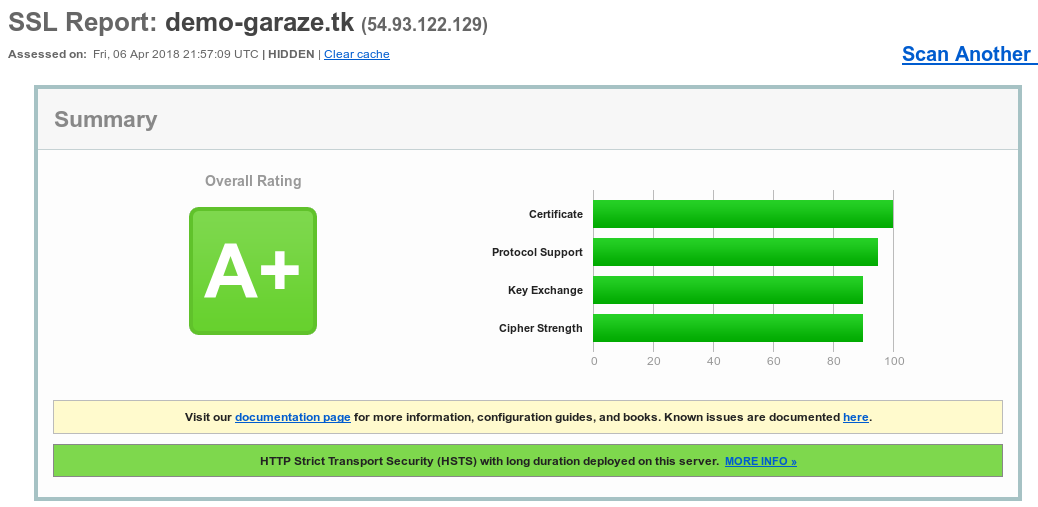
\includegraphics[width=\textwidth]{images/ssl_test.png}
    \caption[Výsledky testu HTTPS konfigurace]{Výsledky testu HTTPS konfigurace poskytnutného společností Qualys.}
    \label{fig:ssl_test}
\end{figure}

% napsat ze sme pri nasazovani prisli na novy chyby, ktery nebyly na lokale videt -- to s tim vodhlasovanim a secret_key, a to ze apache zahazuje ty headery s nepovolenejma znakama
Nasazení aplikace v~reálném prostředí odhalilo několik chyb, které nebyly při lokálním testování patrné. V~první řadě se ukázalo, že server Apache2 od verze 2.4 ignoruje v~příchozím požadavku hlavičky, které obsahují podtržítka \cite{apache_headers_update}. Podtržítka byla původně použita při zasílání hlavičky s~API klíčem (původně \texttt{api\_key}). Tuto chybu jsem opravil přejmenováním hlavičky na \texttt{apikey}.

Druhá chyba se týkala nastavení hodnoty \texttt{secret\_key} v~konfiguračním souboru aplikace. Tento klíč slouží k~podepisování HTTP relace či generování CSRF \textit{tokenů} \cite{flask_api}. V~konfiguraci aplikace použité při lokálním testování byl klíč vždy nastaven na náhodně vygenerovanou hodnotu.

Po nasazení se ukázalo, že WSGI \cite{python_wsgi} modul použitý pro spárování Python aplikace se serverem Apache2 tuto aplikaci v~některých případech restartuje. To by obecně ničemu nevadilo, nicméně při každém restartu byla znovu vygenerována nová hodnota \texttt{secret\_key}, což vedlo k~zneplatnění všech aktivních HTTP relací a CSRF \textit{tokenů}. Uživatel rozhraní tak byl náhle odhlášen nebo nemohl odesílat formuláře. 

V~konfiguračním souboru aplikace, který je použit při jejím nasazení, bylo proto generování klíče nahrazeno pevnou hodnotou (dostatečně dlouhým náhodně generovaným klíčem, který však není reinicializován při restartu aplikace).

% tady by se este dalo napsat ze sme meli preklep v tim apache konfiguraku a proto to wsgi nebezelo v tim daemon modu, a proto byly ty restarty vod nej tak casty, viz https://stackoverflow.com/questions/48507267/mod-wsgi-keeps-restarting-flask-app#comment84021510_48507792

% nicmene to ze generovat ten klic pokazdy je taky spatnej napad je taky pravda viz https://stackoverflow.com/questions/27287391/why-not-generate-the-secret-key-every-time-flask-starts

\subsection{Provozní server}

Aplikace byla nasazena na virtuálním serveru ze služby Amazon EC2, s~jedním procesorovým jádrem a 1 GB paměti. Použitý byl operační systém Ubuntu Xenial 16.04.

\section{Simulátor podřízeného systému}

V~rámci testování aplikace nadřazeného systému jsem vytvořil simulátor podřízeného systému. Ten umožňuje snadné zasílání požadavku na API nadřazeného systému, podobně jako by to dělal reálný podřízený systém.

Simulátor je implementován jako jednoduchá stránka, která je součástí webového rozhraní nadřazeného systému. Zasílání požadavků je realizováno pomocí Javascriptu a knihovny jQuery \cite{jquery_about}. 

Stránka simulátoru je přístupná na \texttt{/simulator}, pokud byla aplikace nadřazeného systému spuštěna v~ladícím módu (\texttt{DEBUG = True} v~konfiguračním souboru aplikace).

\section{Test odezvy nadřazeného systému}
\label{sec:te_lat}

V~závěru testování jsem vyzkoušel dobu odezvy nadřazeného systému při nasazení na Raspberry Pi 3. Chtěl jsem ověřit především dobu zpracování události zaslané podřízeným systémem.

Při testu se ukázalo, že doba odezvy roste s~počtem událostí, které byly pro danou garáž zaznamenány. Z~počátku byly zaslané události zpracovány zhruba za 150 až 200 milisekund. Pokud však měla daná garáž v~databázi uloženo již kolem 2000 událostí, vzrostla doba zpracování až na 800 milisekund.

Příčinou byl výchozí způsob, kterým framework SQLAlchemy mapuje databázové záznamy na Python objekty. Problém byl vyřešen dynamickým načítáním záznamů, které je popsáno v~sekci \ref{sec:im_lazy}. Po této úpravě se doba odezvy ustálila na přibližně 200 milisekudnách, bez ohledu na počet zaznamenaných událostí.

% napsat ze sme vodhalili ten problem s lazy loadingem viz http://docs.sqlalchemy.org/en/latest/orm/collections.html, napsat neco v tom smyslu, ze ten normalni loading co tam je je pomalej pro velky kolekce jako sou ty udalosti a ze se musi pouzit trochu jinej pristup. ruzny strategie sou popsany v tim clanku, a ze my sme zvolili to prvni, teda pouziti dynamic loadingu (muzu napsat ze sme este zkouseli noload).

% este napsat ze s tim dynamic loadingem nejde ke kolekci garage.events pristupovat primo, takze sme udelali funkci garage.get_events(event_type=None), ktera nam ten pristup zapouzdri a este s ni muzem filtrovat podle typu

% tzn ten tradeoff je ze ted to garage.events neni primo kolekce ale nakej query object kterej nevobsahuje vsechnny ty eventy, ale to nevadi protoze k tem eventum stejne pristupujem jen pres to get events. Este tam muzem napsat ze misto toho dynamickyho loadovani bysme mohli dat ten noload a nenacitat ty eventy vubec a pak v ty metode get_events misto toho query objectu co vraci to dynamicky loadovani (pres relationship) bysme pouzivali proste tu tridu Event, stylem Event.query... ale tohle ze je takovy cistsi.

% prave ten hlavni problem ty python kolekce je ze se do ni pri tim appendu musej nacist vsechny ty vobjekty, coz je zbytecny a drahy. Kdezto pri tim dynamickym loadu je to nenacita protoze jakoby ten append nepristupuje k python kolekci ale k nakymu tomu query objektu (vytvorenymu zas pres ten relationship).

% este napsat ze bez toho se pridavani udalosti ke garazim ktery jich uz maj moc furt spomalovalo kvuli tomu appendu, takhle je to +- stejny furt i pro mega udalosti.

% tohle vsechno vychazi z toho collections clanku

% nakonec napsat ze se to da este trochu zrychlit pouzitim tech sessions v requests


\begin{conclusion}
	%sem napište závěr Vaší práce
\end{conclusion}

\bibliographystyle{templates/csn690}
\bibliography{mybibliographyfile}

\appendix

\chapter{Seznam použitých zkratek}
\begin{description}
	\item[API]
	\item[HTTP] Graphical user interface
    \item[HTTPS] Graphical user interface
    \item[MQTT] Graphical user interface
    \item[OSI]
    \item[TCP/IP] Graphical user interface
    \item[URL]
\end{description}

\chapter{Obsah přiloženého CD}

\begin{figure}
	\dirtree{%
		.1 readme.txt\DTcomment{stručný popis obsahu CD}.
		.1 exe\DTcomment{adresář se spustitelnou formou implementace}.
		.1 src.
		.2 impl\DTcomment{zdrojové kódy implementace}.
		.2 thesis\DTcomment{zdrojová forma práce ve formátu \LaTeX{}}.
		.1 text\DTcomment{text práce}.
		.2 thesis.pdf\DTcomment{text práce ve formátu PDF}.
		.2 thesis.ps\DTcomment{text práce ve formátu PS}.
	}
\end{figure}

\end{document}
